% In this file you should put the actual content of the blueprint.
% It will be used both by the web and the print version.
% It should *not* include the \begin{document}
%
% If you want to split the blueprint content into several files then
% the current file can be a simple sequence of \input. Otherwise It
% can start with a \section or \chapter for instance.

\chapter{Introduction}

The goal of this project is to formalize Succinct Non-Interactive Arguments of Knowledge (SNARKs) in
Lean. Our focus is on SNARKs based on Interactive Oracle Proofs (IOPs) and variants thereof (i.e.
Polynomial IOPs). We aim to develop a general framework for IOP-based SNARKs with verified, modular
building blocks and transformations. This modular approach enables us to construct complex protocols
from simpler components while ensuring correctness and soundness by construction.

\chapter{Oracle Reductions}\label{chap:oracle_reductions}

\section{The VCVio Library}\label{sec:vcvio}

This library provides a formal framework for reasoning about computations that make \emph{oracle
queries}. Many cryptographic primitives and interactive protocols use oracles to model (or simulate)
external functionality such as random responses, coin flips, or more structured queries. The VCVio
library "lifts" these ideas into a setting where both the abstract specification and concrete
simulation of oracles may be studied, and their probabilistic behavior analyzed.

The main ingredients of the library are as follows:

\begin{definition}[Specification of Oracles]
    \label{def:oracle_spec}
    An oracle specification describes a collection of available oracles, each with its own input and output types. 
    Formally, it's given by an indexed family where each oracle is specified by:
    \begin{itemize}
        \item A domain type (what inputs it accepts)
        \item A range type (what outputs it can produce)
    \end{itemize}
    The indexing allows for potentially infinite collections of oracles, and the specification itself 
    is agnostic to how the oracles actually behave - it just describes their interfaces.
    \lean{OracleSpec}
\end{definition}

Some examples of oracle specifications (and their intended behavior) are as follows:
\begin{itemize}
    \item \verb|emptySpec|: Represents an empty set of oracles
    \item \verb|singletonSpec|: Represents a single oracle available on a singleton index
    \item \verb|coinSpec|: A coin flipping oracle that produces a random Boolean value
    \item \verb|unifSpec|: A family of oracles that for every natural number $n \in \mathbb{N}$ chooses uniformly from the set $\{0, \ldots, n\}$.
\end{itemize}
    \lean{emptySpec, singletonSpec, coinSpec, unifSpec}

We often require extra properties on the domains and ranges of oracles. For example, we may require that the domains and ranges come equipped with decidable equality \lean{OracleSpec.DecidableEq}
or finiteness properties \lean{OracleSpec.FiniteRange}.

\begin{definition}[Oracle Computation]
    \label{def:oracle_computation}
    An oracle computation represents a program that can make oracle queries. It can:
    \begin{itemize}
        \item Return a pure value without making any queries (via \texttt{pure})
        \item Make an oracle query and continue with the response (via \texttt{queryBind})
        \item Signal failure (via \texttt{failure})
    \end{itemize}
    The formal implementation uses a free monad on the inductive type of oracle queries \lean{OracleSpec.OracleQuery} wrapped in an option monad transformer (i.e. \verb|OptionT(FreeMonad(OracleQuery spec))|).
    \lean{OracleComp}
\end{definition}

\begin{definition}[Handling Oracle Queries]
    \label{def:handling_oracle_queries}
    To actually run oracle computations, we need a way to handle (or implement) the oracle queries.
    An oracle implementation consists a mapping from oracle queries to values in another monad. Depending on the monad, this may allow for various interpretations of the oracle queries.
    \lean{QueryImpl}
\end{definition}

\begin{definition}[Probabilistic Semantics of Oracle Computations]
    \label{def:probabilistic_semantics_of_oracle_computations}
    We can view oracle computations as probabilistic programs by considering what happens when 
    oracles respond uniformly at random. This gives rise to a probability distribution over possible 
    outputs (including the possibility of failure). The semantics maps each oracle query to a 
    uniform distribution over its possible responses.
    \lean{OracleComp.evalDist}
\end{definition}

Once we have mapped an oracle computation to a probability distribution, we can define various associated probabilities, such as the probability of failure, or the probability of the output satisfying a given predicate (assuming it does not fail).

\begin{definition}[Simulating Oracle Queries with Other Oracles]
    \label{def:sim_oracle}
    We can simulate complex oracles using simpler ones by providing a translation mechanism. 
    A simulation oracle specifies how to implement queries in one specification using computations 
    in another specification, possibly maintaining additional state information during the simulation.
    % \lean{SimOracle.Stateful}
\end{definition}

\begin{definition}[Logging \& Caching Oracle Queries]
    \label{def:logging_caching_oracle_queries}
    Using the simulation framework, we can add logging and caching behaviors to oracle queries:
    \begin{itemize}
        \item Logging records all queries made during a computation
        \item Caching remembers query responses and reuses them for repeated queries
    \end{itemize}
    These are implemented as special cases of simulation oracles.
    \lean{loggingOracle, cachingOracle}
\end{definition}

\begin{definition}[Random Oracle]
    \label{def:random_oracle}
    A random oracle is implemented as a caching oracle that uses lazy sampling:
    \begin{itemize}
        \item On first query: generates a uniform random response and caches it
        \item On repeated queries: returns the cached response
    \end{itemize}
    \lean{randomOracle}
\end{definition}

% In summary, the VCVio library consists of:
% \begin{itemize}
%   \item A formal specification of oracles and their inputs/outputs (\texttt{OracleSpec}).
%   \item A monadic framework for computations that may perform oracle queries (\texttt{OracleComp}).
%   \item Effect handlers that permit the interpretation and simulation of oracle queries via
%         customizable implementations (\texttt{OracleImpl} and \texttt{SimOracle}).
%   \item Denotational semantics based on probability mass functions that allow the quantitative analysis
%         of such computations (\texttt{evalDist}, \texttt{probOutput}, \texttt{probFailure}, \texttt{probEvent}).
%   \item Extensions for logging, caching, and random oracles to support analysis of protocols using such oracles.
% \end{itemize}

\section{Composition of Oracle Reductions}\label{sec:composition_oracle_reductions}

In this section, we describe a suite of composition operators for building secure oracle reductions from simpler secure components. In other words, we define a number of definitions that govern how oracle reductions can be composed to form larger reductions, and how the resulting reduction inherits the security properties of the components.

% The first group of rules changes relations and shared oracles.

% \subsection{Changing Relations and Oracles}

% Here we express the consequence rule.  Namely, if we have an oracle reduction for
% \(\mathcal{R}_1 \implies \mathcal{R}_2\), along with
% \(\mathcal{R}_1' \implies \mathcal{R}_1\) and \(\mathcal{R}_2 \implies \mathcal{R}_2'\),
% then we obtain an oracle reduction for \(\mathcal{R}_1' \implies \mathcal{R}_2'\).

% \[
% \frac{%
%   \begin{array}{c}
%     \Psi; \Theta; \Sigma \vdash \{\mathcal{R}_1\}\; \langle \mathcal{P},\, \mathcal{V},\, \mathcal{E}\rangle^{\mathcal{O}} : \tau \;\{\!\!\{\mathcal{R}_2; \,\mathsf{St};\, \epsilon\}\!\!\} \\[1.5ex]
%     \mathcal{R}_1' \implies \mathcal{R}_1 \\[1.5ex]
%     \mathcal{R}_2 \implies \mathcal{R}_2'
%   \end{array}%
% }{%
%   \Psi; \Theta; \Sigma \vdash \{\mathcal{R}_1'\}\; \langle \mathcal{P},\, \mathcal{V},\, \mathcal{E}\rangle^{\mathcal{O}} : \tau \;\{\!\!\{\mathcal{R}_2'; \,\mathsf{St};\, \epsilon\}\!\!\}
% } \quad \text{(Conseq)}
% \]

% % Lifting shared oracles: if $\mathcal{O}_1 \subset \mathcal{O}_2$, then reductions with $\mathcal{O}_1$ lift to reductions with $\mathcal{O}_2$ with the same security properties

% % Frame rule
% \[
% \frac{%
%   \Psi; \Theta; \Sigma \vdash \{\mathcal{R}_1\} \; \langle\mathcal{P}, \mathcal{V}, \mathcal{E}\rangle^{\mathcal{O}} : \tau \; \{\!\!\{\mathcal{R}_2; \mathsf{St}; \epsilon\}\!\!\}
% }{%
%   \Psi; \Theta; \Sigma \vdash \{\mathcal{R} \times \mathcal{R}_1\} \; \langle\mathcal{P}, \mathcal{V}, \mathcal{E}\rangle^{\mathcal{O}} : \tau \; \{\!\!\{\mathcal{R} \times \mathcal{R}_2; \mathsf{St}; \epsilon\}\!\!\}
% } \quad \text{(Frame)}
% \]

% % Oracle lifting rule
% \[
% \frac{%
%   \begin{array}{c}
%     \Psi; \Theta; \Sigma \vdash \{\mathcal{R}_1\} \; \langle\mathcal{P}, \mathcal{V}, \mathcal{E}\rangle^{\mathcal{O}_1} : \tau \; \{\!\!\{\mathcal{R}_2; \mathsf{St}; \epsilon\}\!\!\} \\[1.5ex]
%     \mathcal{O}_1 \subset \mathcal{O}_2
%   \end{array}%
% }{%
%   \Psi; \Theta; \Sigma \vdash \{\mathcal{R}_1\} \; \langle\mathcal{P}, \mathcal{V}, \mathcal{E}\rangle^{\mathcal{O}_2} : \tau \; \{\!\!\{\mathcal{R}_2; \mathsf{St}; \epsilon\}\!\!\}
% } \quad \text{(Oracle-Lift)}
% \]

% TODO: figure out how the state function needs to change for these rules (they are basically the same, but not exactly)

% \subsection{Sequential Composition}

% The reason why we consider interactive (oracle) reductions at the core of our formalism is that we
% can \emph{compose} these reductions to form larger reductions. Equivalently, we can take a complex
% \emph{interactive (oracle) proof} (which differs only in that it reduces a relation to the
% \emph{trivial} relation that always outputs true) and break it down into a series of smaller
% reductions. The advantage of this approach is that we can prove security properties (completeness
% and soundness) for each of the smaller reductions, and these properties will automatically transfer
% to the larger reductions.

% This section is devoted to the composition of interactive (oracle) reductions, and proofs that the
% resulting reductions inherit the security properties of the two (or more) constituent reductions.

% Sequential composition can be expressed as the folowing rule:

% \[
% \frac{%
%   \begin{array}{c}
%     \Psi; \Theta; \varSigma \vdash \{\mathcal{R}_1\} \; \langle\mathcal{P}_1, \mathcal{V}_1, \mathcal{E}_1\rangle^{\mathcal{O}} : \tau_1 \; \{\!\!\{\mathcal{R}_2; \mathsf{St}_1; \epsilon_1\}\!\!\} \\[1.5ex]
%     \Psi; (\Theta :: \tau_1) ; \varSigma \vdash \{\mathcal{R}_2\} \; \langle\mathcal{P}_2, \mathcal{V}_2, \mathcal{E}_2\rangle^{\mathcal{O}} : \tau_2 \; \{\!\!\{\mathcal{R}_3; \mathsf{St}_2; \epsilon_2\}\!\!\}
%   \end{array}%
% }{%
%   \Psi; (\Theta :: \tau_1 :: \tau_2) \ ; \varSigma \vdash \{\mathcal{R}_1\} \; \langle\mathcal{P}_1 \circ \mathcal{P}_2, \mathcal{V}_1 \circ \mathcal{V}_2, \mathcal{E}_1 \circ_{\mathcal{V}_2} \mathcal{E}_2\rangle^{\mathcal{O}} : \tau_1 \oplus \tau_2 \; \{\!\!\{\mathcal{R}_3; \mathsf{St}_1 \oplus \mathsf{St}_2; \epsilon_1 \oplus \epsilon_2\}\!\!\}
% } \quad \text{(Seq-Comp)}
% \]

% % \begin{definition}[Sequential Composition of Protocol Type Signatures]
% %     \label{def:protocol_spec_composition}
% %     \lean{ProtocolSpec.append}
% % \end{definition}

% % \begin{definition}[Sequential Composition of Provers]
% %     \label{def:prover_composition}
% %     \lean{Prover.append}
% % \end{definition}

% % \begin{definition}[Sequential Composition of Oracle Verifiers]
% %     \label{def:oracle_verifier_composition}
% %     \lean{OracleVerifier.append}
% % \end{definition}

% % \begin{definition}[Sequential Composition of Oracle Reductions]
% %     \label{def:oracle_reduction_composition}
% %     \lean{Reduction.append}
% % \end{definition}

\subsection{Sequential Composition}\label{sec:sequential_composition}

Sequential composition allows us to chain together oracle reductions where the output context of one reduction becomes the input context of the next reduction. This is fundamental for building complex protocols from simpler components.

\subsubsection{Composition of Protocol Specifications}

We begin by defining how to compose protocol specifications and their associated structures.

\begin{definition}[Protocol Specification Append]
    \label{def:protocol_spec_append}
    Given two protocol specifications $\pSpec_1 : \ProtocolSpec\ m$ and $\pSpec_2 : \ProtocolSpec\ n$, their sequential composition is:
    \[ \pSpec_1 \mathrel{++_\mathsf{p}} \pSpec_2 : \ProtocolSpec\ (m + n) \]
    \lean{ProtocolSpec.append}
    \uses{def:protocol_spec}
\end{definition}

\begin{definition}[Full Transcript Append]
    \label{def:transcript_append}
    Given full transcripts $T_1 : \FullTranscript\ \pSpec_1$ and $T_2 : \FullTranscript\ \pSpec_2$, their sequential composition is:
    \[ T_1 \mathrel{++_\mathsf{t}} T_2 : \FullTranscript\ (\pSpec_1 \mathrel{++_\mathsf{p}} \pSpec_2) \]
    \lean{ProtocolSpec.FullTranscript.append}
    \uses{def:transcript}
\end{definition}

\subsubsection{Composition of Provers and Verifiers}

\begin{definition}[Prover Append]
    \label{def:prover_append}
    Given provers $P_1 : \Prover\ \pSpec_1\ \oSpec\ \StmtIn_1\ \WitIn_1\ \StmtOut_1\ \WitOut_1$ and $P_2 : \Prover\ \pSpec_2\ \oSpec\ \StmtOut_1\ \WitOut_1\ \StmtOut_2\ \WitOut_2$, their sequential composition is:
    \[ P_1.\append\ P_2 : \Prover\ (\pSpec_1 \mathrel{++_\mathsf{p}} \pSpec_2)\ \oSpec\ \StmtIn_1\ \WitIn_1\ \StmtOut_2\ \WitOut_2 \]

    The composed prover works by:
    \begin{itemize}
        \item Running $P_1$ on the input context to produce an intermediate context
        \item Using this intermediate context as input to $P_2$
        \item Outputting the final context from $P_2$
    \end{itemize}
    \lean{Prover.append}
    \uses{def:prover, def:protocol_spec_append}
\end{definition}

\begin{definition}[Verifier Append]
    \label{def:verifier_append}
    Given verifiers $V_1 : \Verifier\ \pSpec_1\ \oSpec\ \StmtIn_1\ \StmtOut_1$ and $V_2 : \Verifier\ \pSpec_2\ \oSpec\ \StmtOut_1\ \StmtOut_2$, their sequential composition is:
    \[ V_1.\append\ V_2 : \Verifier\ (\pSpec_1 \mathrel{++_\mathsf{p}} \pSpec_2)\ \oSpec\ \StmtIn_1\ \StmtOut_2 \]

    The composed verifier first runs $V_1$ on the first part of the transcript, then runs $V_2$ on the second part using the intermediate statement from $V_1$.
    \lean{Verifier.append}
    \uses{def:verifier, def:protocol_spec_append}
\end{definition}

\begin{definition}[Reduction Append]
    \label{def:reduction_append}
    Sequential composition of reductions combines the corresponding provers and verifiers:
    \[ R_1.\append\ R_2 : \Reduction\ (\pSpec_1 \mathrel{++_\mathsf{p}} \pSpec_2)\ \oSpec\ \StmtIn_1\ \WitIn_1\ \StmtOut_2\ \WitOut_2 \]
    \lean{Reduction.append}
    \uses{def:reduction, def:prover_append, def:verifier_append}
\end{definition}

\begin{definition}[Oracle Reduction Append]
    \label{def:oracle_reduction_append}
    Sequential composition extends naturally to oracle reductions by composing the oracle provers and oracle verifiers.
    \lean{OracleReduction.append}
    \uses{def:oracle_reduction, def:prover_append, def:verifier_append}
\end{definition}

\subsubsection{General Sequential Composition}

For composing an arbitrary number of reductions, we provide a general composition operation.

\begin{definition}[General Protocol Specification Composition]
    \label{def:protocol_spec_compose}
    Given a family of protocol specifications $\pSpec : \forall i : \Fin(m+1), \ProtocolSpec\ (n\ i)$, their composition is:
    \[ \compose\ m\ n\ \pSpec : \ProtocolSpec\ (\sum_{i} n\ i) \]
    \lean{ProtocolSpec.seqCompose}
    \uses{def:protocol_spec}
\end{definition}

\begin{definition}[General Prover Composition]
    \label{def:prover_compose}
    \lean{Prover.seqCompose}
    \uses{def:prover, def:protocol_spec_compose}
\end{definition}

\begin{definition}[General Verifier Composition]
    \label{def:verifier_compose}
    \lean{Verifier.seqCompose}
    \uses{def:verifier, def:protocol_spec_compose}
\end{definition}

\begin{definition}[General Reduction Composition]
    \label{def:reduction_compose}
    \lean{Reduction.seqCompose}
    \uses{def:reduction, def:prover_compose, def:verifier_compose}
\end{definition}

\subsubsection{Security Properties of Sequential Composition}

The key insight is that security properties are preserved under sequential composition.

\begin{theorem}[Completeness Preservation under Append]
    \label{thm:completeness_append}
    If reductions $R_1$ and $R_2$ satisfy completeness with compatible relations and respective errors $\epsilon_1$ and $\epsilon_2$, then their sequential composition $R_1.\append\ R_2$ satisfies completeness with error $\epsilon_1 + \epsilon_2$.
    \lean{Reduction.completeness_append}
    \uses{def:completeness, def:reduction_append}
\end{theorem}

\begin{theorem}[Perfect Completeness Preservation under Append]
    \label{thm:perfect_completeness_append}
    If reductions $R_1$ and $R_2$ satisfy perfect completeness with compatible relations, then their sequential composition also satisfies perfect completeness.
    \lean{Reduction.perfectCompleteness_append}
    \uses{def:perfect_completeness, def:reduction_append}
\end{theorem}

\begin{theorem}[Soundness Preservation under Append]
    \label{thm:soundness_append}
    If verifiers $V_1$ and $V_2$ satisfy soundness with respective errors $\epsilon_1$ and $\epsilon_2$, then their sequential composition satisfies soundness with error $\epsilon_1 + \epsilon_2$.
    \lean{Verifier.append_soundness}
    \uses{def:soundness, def:verifier_append}
\end{theorem}

\begin{theorem}[Knowledge Soundness Preservation under Append]
    \label{thm:knowledge_soundness_append}
    If verifiers $V_1$ and $V_2$ satisfy knowledge soundness with respective errors $\epsilon_1$ and $\epsilon_2$, then their sequential composition satisfies knowledge soundness with error $\epsilon_1 + \epsilon_2$.
    \lean{Verifier.append_knowledgeSoundness}
    \uses{def:knowledge_soundness, def:verifier_append}
\end{theorem}

\begin{theorem}[Round-by-Round Soundness Preservation under Append]
    \label{thm:rbr_soundness_append}
    If verifiers $V_1$ and $V_2$ satisfy round-by-round soundness, then their sequential composition also satisfies round-by-round soundness.
    \lean{Verifier.append_rbrSoundness}
    \uses{def:round_by_round_soundness, def:verifier_append}
\end{theorem}

\begin{theorem}[Round-by-Round Knowledge Soundness Preservation under Append]
    \label{thm:rbr_knowledge_soundness_append}
    If verifiers $V_1$ and $V_2$ satisfy round-by-round knowledge soundness, then their sequential composition also satisfies round-by-round knowledge soundness.
    \lean{Verifier.append_rbrKnowledgeSoundness}
    \uses{def:round_by_round_knowledge_soundness, def:verifier_append}
\end{theorem}

Similar preservation theorems hold for the general composition of multiple reductions:

\begin{theorem}[General Completeness Preservation]
    \label{thm:completeness_compose}
    \lean{Reduction.completeness_seqCompose}
    \uses{def:completeness, def:reduction_compose}
\end{theorem}

\begin{theorem}[General Soundness Preservation]
    \label{thm:soundness_compose}
    \lean{Verifier.seqCompose_soundness}
    \uses{def:soundness, def:verifier_compose}
\end{theorem}

\begin{theorem}[General Knowledge Soundness Preservation]
    \label{thm:knowledge_soundness_compose}
    \lean{Verifier.seqCompose_knowledgeSoundness}
    \uses{def:knowledge_soundness, def:verifier_compose}
\end{theorem}

\subsection{Lifting Contexts}\label{sec:lifting_contexts}

Another essential tool for modular oracle reductions is the ability to adapt reductions from one context to another. This allows us to apply reductions designed for simple contexts to more complex scenarios.

\subsubsection{Context Lenses}

The fundamental abstraction for context adaptation is a \emph{context lens}, which provides bidirectional mappings between outer and inner contexts.

\begin{definition}[Statement Lens]
    \label{def:statement_lens}
    A statement lens between outer context types $(\StmtIn_{\mathsf{outer}}, \StmtOut_{\mathsf{outer}})$ and inner context types $(\StmtIn_{\mathsf{inner}}, \StmtOut_{\mathsf{inner}})$ consists of:
    \begin{itemize}
        \item $\projStmt : \StmtIn_{\mathsf{outer}} \to \StmtIn_{\mathsf{inner}}$ (projection to inner context)
        \item $\liftStmt : \StmtIn_{\mathsf{outer}} \times \StmtOut_{\mathsf{inner}} \to \StmtOut_{\mathsf{outer}}$ (lifting back to outer context)
    \end{itemize}
    \lean{Statement.Lens}
\end{definition}

\begin{definition}[Witness Lens]
    \label{def:witness_lens}
    A witness lens between outer witness types $(\WitIn_{\mathsf{outer}}, \WitOut_{\mathsf{outer}})$ and inner witness types $(\WitIn_{\mathsf{inner}}, \WitOut_{\mathsf{inner}})$ consists of:
    \begin{itemize}
        \item $\projWit : \WitIn_{\mathsf{outer}} \to \WitIn_{\mathsf{inner}}$ (projection to inner context)
        \item $\liftWit : \WitIn_{\mathsf{outer}} \times \WitOut_{\mathsf{inner}} \to \WitOut_{\mathsf{outer}}$ (lifting back to outer context)
    \end{itemize}
    \lean{Witness.Lens}
\end{definition}

\begin{definition}[Context Lens]
    \label{def:context_lens}
    A context lens combines a statement lens and a witness lens for adapting complete reduction contexts.
    \lean{Context.Lens}
    \uses{def:statement_lens, def:witness_lens}
\end{definition}

\begin{definition}[Oracle Context Lens]
    \label{def:oracle_context_lens}
    For oracle reductions, we additionally need lenses for oracle statements that can simulate oracle access between contexts.
    \lean{OracleContext.Lens}
    \uses{def:context_lens, def:oracle_interface}
\end{definition}

\subsubsection{Lifting Reductions}

Given a context lens, we can lift reductions from inner contexts to outer contexts.

\begin{definition}[Prover Context Lifting]
    \label{def:prover_lift_context}
    Given a prover $P$ for the inner context and a context lens, the lifted prover works by:
    \begin{itemize}
        \item Projecting the outer input to the inner context
        \item Running the inner prover
        \item Lifting the output back to the outer context
    \end{itemize}
    \lean{Prover.liftContext}
    \uses{def:prover, def:context_lens}
\end{definition}

\begin{definition}[Verifier Context Lifting]
    \label{def:verifier_lift_context}
    \lean{Verifier.liftContext}
    \uses{def:verifier, def:statement_lens}
\end{definition}

\begin{definition}[Reduction Context Lifting]
    \label{def:reduction_lift_context}
    \lean{Reduction.liftContext}
    \uses{def:reduction, def:prover_lift_context, def:verifier_lift_context}
\end{definition}

\subsubsection{Conditions for Security Preservation}

For lifting to preserve security properties, the context lens must satisfy certain conditions.

\begin{definition}[Completeness-Preserving Context Lens]
    \label{def:context_lens_is_complete}
    A context lens preserves completeness if it maintains relation satisfaction under projection and lifting.
    \lean{Context.Lens.IsComplete}
    \uses{def:context_lens}
\end{definition}

\begin{definition}[Soundness-Preserving Statement Lens]
    \label{def:statement_lens_is_sound}
    A statement lens preserves soundness if it maps invalid statements to invalid statements.
    \lean{Statement.Lens.IsSound}
    \uses{def:statement_lens}
\end{definition}

\begin{definition}[RBR Soundness-Preserving Statement Lens]
    \label{def:statement_lens_is_rbr_sound}
    For round-by-round soundness, we need a slightly relaxed soundness condition.
    \lean{Statement.Lens.IsSound}
    \uses{def:statement_lens}
\end{definition}

\begin{definition}[Knowledge Soundness-Preserving Context Lens]
    \label{def:context_lens_is_knowledge_sound}
    A context lens preserves knowledge soundness if it maintains witness extractability.
    \lean{Extractor.Lens.IsKnowledgeSound}
    \uses{def:context_lens}
\end{definition}

\subsubsection{Security Preservation Theorems for Context Lifting}

\begin{theorem}[Completeness Preservation under Context Lifting]
    \label{thm:lift_context_completeness}
    If a reduction satisfies completeness and the context lens is completeness-preserving, then the lifted reduction also satisfies completeness.
    \lean{Reduction.liftContext_completeness}
    \uses{def:completeness, def:reduction_lift_context, def:context_lens_is_complete}
\end{theorem}

\begin{theorem}[Soundness Preservation under Context Lifting]
    \label{thm:lift_context_soundness}
    If a verifier satisfies soundness and the statement lens is soundness-preserving, then the lifted verifier also satisfies soundness.
    \lean{Verifier.liftContext_soundness}
    \uses{def:soundness, def:verifier_lift_context, def:statement_lens_is_sound}
\end{theorem}

\begin{theorem}[Knowledge Soundness Preservation under Context Lifting]
    \label{thm:lift_context_knowledge_soundness}
    If a verifier satisfies knowledge soundness and the context lens is knowledge soundness-preserving, then the lifted verifier also satisfies knowledge soundness.
    \lean{Verifier.liftContext_knowledgeSoundness}
    \uses{def:knowledge_soundness, def:verifier_lift_context, def:context_lens_is_knowledge_sound}
\end{theorem}

\begin{theorem}[RBR Soundness Preservation under Context Lifting]
    \label{thm:lift_context_rbr_soundness}
    If a verifier satisfies round-by-round soundness and the statement lens is RBR soundness-preserving, then the lifted verifier also satisfies round-by-round soundness.
    \lean{Verifier.liftContext_rbr_soundness}
    \uses{def:round_by_round_soundness, def:verifier_lift_context, def:statement_lens_is_rbr_sound}
\end{theorem}

\begin{theorem}[RBR Knowledge Soundness Preservation under Context Lifting]
    \label{thm:lift_context_rbr_knowledge_soundness}
    If a verifier satisfies round-by-round knowledge soundness and the context lens is knowledge soundness-preserving, then the lifted verifier also satisfies round-by-round knowledge soundness.
    \lean{Verifier.liftContext_rbr_knowledgeSoundness}
    \uses{def:round_by_round_knowledge_soundness, def:verifier_lift_context, def:context_lens_is_knowledge_sound}
\end{theorem}

\subsubsection{Extractors and State Functions}

Context lifting also applies to extractors and state functions used in knowledge soundness and round-by-round soundness.

\begin{definition}[Straightline Extractor Lifting]
    \label{def:straightline_extractor_lift_context}
    \lean{Extractor.Straightline.liftContext}
    \uses{def:straightline_extractor, def:context_lens}
\end{definition}

\begin{definition}[Round-by-Round Extractor Lifting]
    \label{def:rbr_extractor_lift_context}
    \lean{Extractor.RoundByRound.liftContext}
    \uses{def:rbr_extractor, def:context_lens}
\end{definition}

\begin{definition}[State Function Lifting]
    \label{def:state_function_lift_context}
    \lean{Verifier.StateFunction.liftContext}
    \uses{def:state_function, def:statement_lens}
\end{definition}

These composition and lifting operators provide the essential building blocks for constructing complex oracle reductions from simpler components while preserving their security properties.

% \subsection{Virtualization}

% Another tool we will repeatedly use is the ability to change the context of an oracle reduction. This is often needed when we want to adapt an oracle reduction in a simple context into one for a more complex context.

% See the section on sum-check~\ref{sec:sumcheck} for an example.

% \begin{definition}[Mapping into Virtual Context]
%     \label{def:virtual_context_mapping}
%     In order to apply an oracle reduction on virtual data, we will need to provide a mapping from the current context to the virtual context. This includes:
%     \begin{itemize}
%         \item A mapping from the current public inputs to the virtual public inputs.
%         \item A simulation of the oracle inputs for the virtual context using the public and oracle
%         inputs for the current context.
%         \item A mapping from the current private inputs to the virtual private inputs.
%         \item A simulation of the shared oracle for the virtual context using the shared oracle for
%         the current context.
%     \end{itemize}
% \end{definition}

% \begin{definition}[Virtual Oracle Reduction]
%     \label{def:virtual_oracle_reduction}
%     Given a suitable mapping into a virtual context, we may define an oracle reduction via the following construction:
%     \begin{itemize}
%         \item The prover first applies the mappings to obtain the virtual context. The verifier does the same, but only for the non-private inputs.
%         \item The prover and verifier then run the virtual oracle reduction on the virtual context.
%     \end{itemize}
% \end{definition}

% We will show security properties for this virtualization process. One can see that completeness and soundness are inherited from the completeness and soundness of the virtual oracle reduction. However, (round-by-round) knowledge soundness is more tricky; this is because we must extract back to the witness of the original context from the virtual context.

% % virtual-ctx rule of the form: if we have an oracle reduction from R1 to R2 for context prime, a mapping `f` from ctx to ctx prime, and an inverse mapping `g` from witness of ctx prime to witness of ctx, then we have an oracle reduction from (R1 \circ f) to (R2 \circ g) for ctx. The prover & verifier & the state function are composed with `f`, and the extractor needs to be composed with both `f` and `g`.

% % Virtualization rule
% \[
% \frac{%
%   \begin{array}{c}
%     \Psi'; \Theta'; \Sigma' \vdash \{\mathcal{R}_1\} \; \langle\mathcal{P}, \mathcal{V}, \mathcal{E}\rangle^{\mathcal{O}} : \tau \; \{\!\!\{\mathcal{R}_2; \mathsf{St}; \epsilon\}\!\!\} \\[1.5ex]
%     f : (\Psi, \Theta, \Sigma) \to (\Psi', \Theta', \Sigma') \\[1.5ex]
%     g : \Psi' \to \Psi \\[1.5ex]
%     f.\mathsf{fst} \circ g = \mathsf{id}
%   \end{array}%
% }{%
%   \Psi; \Theta; \Sigma \vdash \{\mathcal{R}_1 \circ f\} \; \langle\mathcal{P} \circ f, \mathcal{V} \circ f, \mathcal{E} \circ (f, g)\rangle^{\mathcal{O}} : \tau \; \{\!\!\{\mathcal{R}_2 \circ f; \mathsf{St} \circ f; \epsilon\}\!\!\}
% } \quad \text{(Virtual-Ctx)}
% \]

% \subsection{Substitution}

% Finally, we need a transformation / inference rule that allows us to change the message type in a given round of an oracle reduction. In other words, we substitute a value in the round with another value, followed by a reduction establishing the relationship between the new and old values.

% % May need multiple rules for different types of substitutions (i.e. whether in context or in protocol type, where replacing oracle / public message with oracle / public / private message, etc.)

% Examples include:
% \begin{enumerate}
%     \item Substituting an oracle input by a public input:
%     \begin{itemize}
%         \item Often by just revealing the underlying data. This has no change on the prover, and for
%         the verifier, this means that any query to the oracle input can be locally computed.
%         \item A variant of this is when the oracle input consists of a data along with a proof that
%         the data satisfies some predicate. In this case, the verifier needs to additionally check
%         that the predicate holds for the substituted data.
%         \item Another common substitution is to replace a vector with its Merkle commitment, or a
%         polynomial with its polynomial commitment.
%     \end{itemize}
%     \item Substituting an oracle input by another oracle input, followed by a reduction for each
%     oracle query the verifier makes to the old oracle:
%     \begin{itemize}
%         \item This is also a variant of the previous case, where we do not fully substitute with a
%         public input, but do a ``half-substitution'' by substituting with another oracle input. This
%         happens e.g. when using a polynomial commitment scheme that is itself based on a vector
%         commitment scheme. One can cast protocols like Ligero / Brakedown / FRI / STIR in this
%         two-step process.
%     \end{itemize}
% \end{enumerate}


\chapter{Proof Systems}\label{chap:proof_systems}

\section{Simple Oracle Reductions}

We start by introducing a number of simple oracle reductions that serve as fundamental building blocks for more complex proof systems. These components can be composed together to construct larger protocols.

\subsection{Trivial Reduction}

The simplest possible oracle reduction is one that performs no computation at all. Both the prover and verifier simply pass their inputs through unchanged. While seemingly trivial, this reduction serves as an important identity element for composition and provides a base case for lifting and lens operations.

\begin{definition}[DoNothing Reduction]
    \label{def:donothing_reduction}
    The DoNothing reduction is a zero-round protocol with the following components:
    \begin{itemize}
        \item \textbf{Protocol specification}: $\pSpec := []$ (empty protocol, no messages exchanged)
        \item \textbf{Prover}: Simply stores the input statement and witness, and outputs them unchanged
        \item \textbf{Verifier}: Takes the input statement and outputs it directly
        \item \textbf{Input relation}: Any relation $R_{\mathsf{in}} : \StmtIn \to \WitIn \to \Prop$
        \item \textbf{Output relation}: The same relation $R_{\mathsf{out}} := R_{\mathsf{in}}$
    \end{itemize}
    \lean{DoNothing.reduction, DoNothing.oracleReduction}
\end{definition}

\begin{theorem}[DoNothing Perfect Completeness]
    The DoNothing reduction satisfies perfect completeness for any input relation.
    \lean{DoNothing.reduction_perfectCompleteness, DoNothing.oracleReduction_perfectCompleteness}
    \uses{def:donothing_reduction}
\end{theorem}

The oracle version of DoNothing handles oracle statements by passing them through unchanged as well. The prover receives both non-oracle and oracle statements as input, and outputs them in the same form to the verifier.

\subsection{Sending the Witness}

A fundamental building block in many proof systems is the ability for the prover to transmit witness information to the verifier. The SendWitness reduction provides this functionality in both direct and oracle settings.

\begin{definition}[SendWitness Reduction]
    \label{def:sendwitness_reduction}
    The SendWitness reduction is a one-round protocol where the prover sends the complete witness to the verifier:
    \begin{itemize}
        \item \textbf{Protocol specification}: $\pSpec := [(\PtoVdir, \WitIn)]$ (single message from prover to verifier)
        \item \textbf{Prover}: Sends the witness $\mathbbm{w}$ as its single message
        \item \textbf{Verifier}: Receives the witness and combines it with the input statement to form the output
        \item \textbf{Input relation}: $R_{\mathsf{in}} : \StmtIn \to \WitIn \to \Prop$
        \item \textbf{Output relation}: $R_{\mathsf{out}} : (\StmtIn \times \WitIn) \to \Unit \to \Prop$ defined by $((\mathsf{stmt}, \mathsf{wit}), ()) \mapsto R_{\mathsf{in}}(\mathsf{stmt}, \mathsf{wit})$
    \end{itemize}
    \lean{SendWitness.reduction}
    \uses{def:reduction}
\end{definition}

\begin{theorem}[SendWitness Perfect Completeness]
    The SendWitness reduction satisfies perfect completeness.
    \lean{SendWitness.reduction_completeness}
    \uses{def:sendwitness_reduction}
\end{theorem}

In the oracle setting, we consider two variants:

\begin{definition}[SendWitness Oracle Reduction]
    \label{def:sendwitness_oracle_reduction}
    The oracle version handles witnesses that are indexed families of types with oracle interfaces:
    \begin{itemize}
        \item \textbf{Witness type}: $\WitIn : \iota_w \to \Type$ where each $\WitIn(i)$ has an oracle interface
        \item \textbf{Protocol specification}: $\pSpec := [(\PtoVdir, \forall i, \WitIn(i))]$
        \item \textbf{Output oracle statements}: Combination of input oracle statements and the transmitted witness
    \end{itemize}
    % \lean{SendWitness.oracleReduction}
    \uses{def:oracle_reduction}
\end{definition}

\begin{definition}[SendSingleWitness Oracle Reduction]
    \label{def:sendsinglewitness_oracle_reduction}
    A specialized variant for a single witness with oracle interface:
    \begin{itemize}
        \item \textbf{Witness type}: $\WitIn : \Type$ with oracle interface
        \item \textbf{Protocol specification}: $\pSpec := [(\PtoVdir, \WitIn)]$
        \item \textbf{Conversion}: Implicitly converts to indexed family $\WitIn : \Fin(1) \to \Type$
    \end{itemize}
    \lean{SendSingleWitness.oracleReduction}
\end{definition}

\begin{theorem}[SendSingleWitness Perfect Completeness]
    The SendSingleWitness oracle reduction satisfies perfect completeness.
    \lean{SendSingleWitness.oracleReduction_completeness}
    \uses{def:sendsinglewitness_oracle_reduction}
\end{theorem}

\subsection{Oracle Equality Testing}

One of the most fundamental oracle reductions is testing whether two oracles of the same type are equal. This is achieved through random sampling from the query space.

\begin{definition}[RandomQuery Oracle Reduction]
    \label{def:randomquery_oracle_reduction}
    The RandomQuery reduction tests equality between two oracles by random querying:
    \begin{itemize}
        \item \textbf{Input}: Two oracles $\mathsf{a}, \mathsf{b}$ of the same type with oracle interface
        \item \textbf{Protocol specification}: $\pSpec := [(\VtoPdir, \mathsf{Query})]$ (single challenge from verifier)
        \item \textbf{Input relation}: $R_{\mathsf{in}}((), (\mathsf{a}, \mathsf{b}), ()) := (\mathsf{a} = \mathsf{b})$
        \item \textbf{Verifier}: Samples random query $q$ and sends it to prover
        \item \textbf{Prover}: Receives query $q$, performs no computation
        \item \textbf{Output relation}: $R_{\mathsf{out}}((q, (\mathsf{a}, \mathsf{b})), ()) := (\mathsf{oracle}(\mathsf{a}, q) = \mathsf{oracle}(\mathsf{b}, q))$
    \end{itemize}
    \lean{RandomQuery.oracleReduction}
    \uses{def:oracle_reduction}
\end{definition}

\begin{theorem}[RandomQuery Perfect Completeness]
    The RandomQuery oracle reduction satisfies perfect completeness: if two oracles are equal, they will agree on any random query.
    \lean{RandomQuery.oracleReduction_completeness}
    \uses{def:randomquery_oracle_reduction}
\end{theorem}

The key security property of RandomQuery depends on the notion of oracle distance:

\begin{definition}[Oracle Distance]
    \label{def:oracle_distance}
    For oracles $\mathsf{a}, \mathsf{b}$ of the same type, we define their distance as:
    \[ \mathsf{distance}(\mathsf{a}, \mathsf{b}) := |\{q : \mathsf{Query} \mid \mathsf{oracle}(\mathsf{a}, q) \neq \mathsf{oracle}(\mathsf{b}, q)\}| \]

    We say an oracle type has distance bound $d$ if for any two distinct oracles $\mathsf{a} \neq \mathsf{b}$, we have $\mathsf{distance}(\mathsf{a}, \mathsf{b}) \geq |\mathsf{Query}| - d$.
\end{definition}

\begin{theorem}[RandomQuery Knowledge Soundness]
    If the oracle type has distance bound $d$, then the RandomQuery oracle reduction satisfies round-by-round knowledge soundness with error probability $\frac{d}{|\mathsf{Query}|}$.
    \lean{RandomQuery.oracleVerifier_rbrKnowledgeSoundness}
    \uses{def:randomquery_oracle_reduction, def:oracle_distance}
\end{theorem}

\begin{definition}[RandomQueryWithResponse Variant]
    \label{def:randomquery_with_response}
    A variant of RandomQuery where the second oracle is replaced with an explicit response:
    \begin{itemize}
        \item \textbf{Input}: Single oracle $\mathsf{a}$ and target response $r$
        \item \textbf{Output relation}: $R_{\mathsf{out}}(((q, r), \mathsf{a}), ()) := (\mathsf{oracle}(\mathsf{a}, q) = r)$
    \end{itemize}
    This variant is useful when one wants to verify a specific query-response pair rather than oracle equality.
    % \lean{RandomQueryWithResponse}
    \uses{def:randomquery_oracle_reduction}
\end{definition}

We mention two special cases of RandomQuery that are useful for specific applications.

\subsubsection{Polynomial Equality Testing}

A common application of oracle reductions is testing equality between polynomial oracles. This is a specific instance of the RandomQuery reduction applied to polynomial evaluation oracles.

\begin{definition}[Polynomial Equality Testing]
    \label{def:polynomial_equality_testing}
    Consider two univariate polynomials $P, Q \in \mathbb{F}[X]$ of degree at most $d$, available as polynomial evaluation oracles. The polynomial equality testing reduction is defined as:
    \begin{itemize}
        \item \textbf{Input relation}: $P = Q$ as polynomials
        \item \textbf{Protocol specification}: Single challenge of type $\mathbb{F}$ from verifier to prover
        \item \textbf{Honest prover}: Receives the random field element $r$ but performs no computation
        \item \textbf{Honest verifier}: Checks that $P(r) = Q(r)$ by querying both polynomial oracles
        \item \textbf{Output relation}: $P(r) = Q(r)$ for the sampled point $r$
    \end{itemize}
\end{definition}

\begin{theorem}[Polynomial Equality Testing Completeness]
    The polynomial equality testing reduction satisfies perfect completeness: if $P = Q$ as polynomials, then $P(r) = Q(r)$ for any field element $r$.
\end{theorem}

\begin{theorem}[Polynomial Equality Testing Soundness]
    The polynomial equality testing reduction satisfies round-by-round knowledge soundness with error probability $\frac{d}{|\mathbb{F}|}$, where $d$ is the maximum degree bound. This follows from the Schwartz-Zippel lemma: distinct polynomials of degree at most $d$ can agree on at most $d$ points.
\end{theorem}

The state function for this reduction corresponds precisely to the input and output relations, transitioning from checking polynomial equality to checking evaluation equality at the sampled point.

\subsubsection{Batching Polynomial Evaluation Claims}

Another important building block is the ability to batch multiple polynomial evaluation claims into a single check using random linear combinations.

TODO: express this as a lifted version of $\mathsf{RandomQuery}$ over a virtual polynomial whose
variables are the random linear combination coefficients.

\begin{definition}[Batching Polynomial Evaluation Claims]
    \label{def:batching_polynomial_evaluation}
    Consider an $n$-tuple of values $v = (v_1, \ldots, v_n) \in \mathbb{F}^n$ and a polynomial map $E : \mathbb{F}^k \to \mathbb{F}^n$. The batching reduction is defined as:
    \begin{itemize}
        \item \textbf{Protocol specification}: Two messages:
        \begin{enumerate}
            \item Verifier sends random $r \in \mathbb{F}^k$ to prover
            \item Prover sends $\langle E(r), v \rangle := \sum_{i=1}^n E(r)_i \cdot v_i$ to verifier
        \end{enumerate}
        \item \textbf{Honest prover}: Computes the inner product $\langle E(r), v \rangle$ and sends it
        \item \textbf{Honest verifier}: Verifies that the received value equals the expected inner product
        \item \textbf{Extractor}: Trivial since there is no witness to extract
    \end{itemize}
\end{definition}

\begin{theorem}[Batching Completeness]
    The batching polynomial evaluation reduction satisfies perfect completeness.
\end{theorem}

\begin{remark}[Batching Security]
    The security of this reduction depends on the degree and non-degeneracy properties of the polynomial map $E$. The specific error bounds depend on the structure of $E$ and require careful analysis of the polynomial's properties.
\end{remark}

\subsection{Sending a Claim}

The SendClaim reduction enables a prover to transmit a claim (oracle statement) to the verifier, who then verifies a relationship between the original and transmitted claims.

\begin{definition}[SendClaim Oracle Reduction]
    \label{def:sendclaim_oracle_reduction}
    The SendClaim reduction is a one-round protocol for claim transmission:
    \begin{itemize}
        \item \textbf{Protocol specification}: $\pSpec := [(\PtoVdir, \OStmtIn)]$ (single oracle message)
        \item \textbf{Input}: Statement and single oracle statement (via $\mathsf{Unique}$ index type)
        \item \textbf{Prover}: Sends the input oracle statement as protocol message
        \item \textbf{Verifier}: Executes oracle computation $\mathsf{relComp} : \StmtIn \to \OracleComp[\OStmtIn]_{\mathcal{O}} \Unit$
        \item \textbf{Output oracle statements}: Sum type $\OStmtIn \oplus \OStmtIn$ containing both original and transmitted claims
        \item \textbf{Output relation}: $R_{\mathsf{out}}((), \mathsf{oracles}) := \mathsf{oracles}(\mathsf{inl}) = \mathsf{oracles}(\mathsf{inr})$
    \end{itemize}
    \lean{SendClaim.oracleReduction}
    \uses{def:oracle_reduction}
\end{definition}

\begin{theorem}[SendClaim Perfect Completeness]
    The SendClaim oracle reduction satisfies perfect completeness when the input relation matches the oracle computation requirement.
    \lean{SendClaim.completeness}
    \uses{def:sendclaim_oracle_reduction}
\end{theorem}

\begin{remark}[SendClaim Development Status]
    The SendClaim reduction is currently under active development in the Lean formalization. Several components including the verifier embedding and completeness proof require further implementation. The current version represents a specialized case that may be generalized in future iterations.
    % TODO: Complete implementation as noted in the Lean code
\end{remark}

\subsection{Claim Reduction}

A fundamental building block for constructing complex proof systems is the ability to locally reduce one type of claim to another. The ReduceClaim reduction provides this functionality through mappings between statement and witness types.

\begin{definition}[ReduceClaim Reduction]
    \label{def:reduceclaim_reduction}
    The ReduceClaim reduction is a zero-round protocol that transforms claims via explicit mappings:
    \begin{itemize}
        \item \textbf{Protocol specification}: $\pSpec := []$ (no messages exchanged)
        \item \textbf{Statement mapping}: $\mathsf{mapStmt} : \StmtIn \to \StmtOut$
        \item \textbf{Witness mapping}: $\mathsf{mapWit} : \WitIn \to \WitOut$
        \item \textbf{Prover}: Applies both mappings to input statement and witness
        \item \textbf{Verifier}: Applies statement mapping to input statement
        \item \textbf{Input relation}: $R_{\mathsf{in}} : \StmtIn \to \WitIn \to \Prop$
        \item \textbf{Output relation}: $R_{\mathsf{out}} : \StmtOut \to \WitOut \to \Prop$
        \item \textbf{Relation condition}: $R_{\mathsf{in}}(\mathsf{stmt}, \mathsf{wit}) \iff R_{\mathsf{out}}(\mathsf{mapStmt}(\mathsf{stmt}), \mathsf{mapWit}(\mathsf{wit}))$
    \end{itemize}
    \lean{ReduceClaim.reduction}
    \uses{def:reduction}
\end{definition}

\begin{theorem}[ReduceClaim Perfect Completeness]
    The ReduceClaim reduction satisfies perfect completeness when the relation condition holds.
    \lean{ReduceClaim.reduction_completeness}
    \uses{def:reduceclaim_reduction}
\end{theorem}

\begin{definition}[ReduceClaim Oracle Reduction]
    \label{def:reduceclaim_oracle_reduction}
    The oracle version additionally handles oracle statements through an embedding:
    \begin{itemize}
        \item \textbf{Oracle statement mapping}: Embedding $\mathsf{embedIdx} : \iota_{\mathsf{out}} \hookrightarrow \iota_{\mathsf{in}}$
        \item \textbf{Type compatibility}: $\OStmtIn(\mathsf{embedIdx}(i)) = \OStmtOut(i)$ for all $i$
        \item \textbf{Oracle embedding}: Maps output oracle indices to corresponding input oracle indices
    \end{itemize}
    \lean{ReduceClaim.oracleReduction}
    \uses{def:oracle_reduction, def:reduceclaim_reduction}
\end{definition}

\begin{remark}[ReduceClaim Oracle Completeness]
    The oracle version's completeness proof is currently under development in the Lean formalization.
    % TODO: Complete when oracleReduction_completeness is implemented
\end{remark}

\subsection{Claim Verification}

Another essential building block is the ability to verify that a given predicate holds for a statement without requiring additional witness information.

\begin{definition}[CheckClaim Reduction]
    \label{def:checkclaim_reduction}
    The CheckClaim reduction is a zero-round protocol that verifies predicates:
    \begin{itemize}
        \item \textbf{Protocol specification}: $\pSpec := []$ (no messages exchanged)
        \item \textbf{Predicate}: $\mathsf{pred} : \StmtIn \to \Prop$ (decidable)
        \item \textbf{Prover}: Simply stores and outputs the input statement with unit witness
        \item \textbf{Verifier}: Checks $\mathsf{pred}(\mathsf{stmt})$ and outputs statement if successful
        \item \textbf{Input relation}: $R_{\mathsf{in}}(\mathsf{stmt}, ()) := \mathsf{pred}(\mathsf{stmt})$
        \item \textbf{Output relation}: $R_{\mathsf{out}}(\mathsf{stmt}, ()) := \mathsf{True}$ (trivial after verification)
    \end{itemize}
    \lean{CheckClaim.reduction}
    \uses{def:reduction}
\end{definition}

\begin{theorem}[CheckClaim Perfect Completeness]
    The CheckClaim reduction satisfies perfect completeness.
    \lean{CheckClaim.reduction_completeness}
    \uses{def:checkclaim_reduction}
\end{theorem}

\begin{definition}[CheckClaim Oracle Reduction]
    \label{def:checkclaim_oracle_reduction}
    The oracle version handles predicates that require oracle access:
    \begin{itemize}
        \item \textbf{Oracle predicate}: $\mathsf{pred} : \StmtIn \to \OracleComp[\OStmtIn]_{\mathcal{O}} \Prop$
        \item \textbf{Never-fails condition}: $\mathsf{pred}(\mathsf{stmt})$ never fails for any statement
        \item \textbf{Oracle computation}: Verifier executes oracle computation to check predicate
        \item \textbf{Input relation}: Defined via oracle simulation of the predicate
    \end{itemize}
    \lean{CheckClaim.oracleReduction}
    \uses{def:oracle_reduction, def:checkclaim_reduction}
\end{definition}

\begin{theorem}[CheckClaim Oracle Perfect Completeness]
    The CheckClaim oracle reduction satisfies perfect completeness.
    \lean{CheckClaim.oracleReduction_completeness}
    \uses{def:checkclaim_oracle_reduction}
\end{theorem}

\begin{remark}[CheckClaim Security Analysis]
    The round-by-round knowledge soundness proofs for both reduction and oracle versions are currently under development in the Lean formalization.
\end{remark}


\section{The Sum-Check Protocol}\label{sec:sumcheck}

In this section, we describe the sum-check protocol~\cite{sumcheck-protocol} in a modular manner, as a running example for our approach to specifying and proving properties of oracle reductions (based on a program logic approach).

The sum-check protocol, as described in the original paper and many expositions thereafter, is a
protocol to reduce the claim that \[ \sum_{x \in \{0, 1\}^n} P(x) = c, \] where $P$ is an
$n$-variate polynomial of certain individual degree bounds, and $c$ is some field element, to the
claim that \[ P(r) = v, \] for some claimed value $v$ (derived from the protocol transcript), where
$r$ is a vector of random challenges from the verifier sent during the protocol.

In our language, the initial context of the sum-check protocol is the pair $(P, c)$, where $P$ is an
oracle input and $c$ is public. The protocol proceeds in $n$ rounds of interaction, where in each
round $i$ the prover sends a univariate polynomial $s_i$ of bounded degree and the verifier sends a
challenge $r_i \gets \mathbb{F}$. The honest prover would compute \[ s_i(X) = \sum_{x \in \{0,
1\}^{n - i - 1}} P(r_1, \ldots, r_{i - 1}, X, x), \] and the honest verifier would check that
$s_i(0) + s_i(1) = s_{i - 1}(r_{i - 1})$, with the convention that $s_0(r_0) = c$.

\begin{theorem}
    The sum-check protocol is complete.
\end{theorem}

We now proceed to break down this protocol into individual message, and then specify the predicates that should hold before and after each message is exchanged.

First, it is clear that we can consider each round in isolation. In fact, each round can be seen as an instantiation of the following simpler "virtual" protocol:
\begin{enumerate}
    \item In this protocol, the context is a pair $(p, d)$, where $p$ is now a \emph{univariate} polynomial of bounded degree. The predicate / relation is that $p(0) + p(1) = d$.
    \item The prover first sends a univariate polynomial $s$ of the same bounded degree as $p$. In
    the honest case, it would just send $p$ itself.
    \item The verifier samples and sends a random challenge $r \gets \mathbb{F}$.
    \item The verifier checks that $s(0) + s(1) = d$. The predicate on the resulting output context
    is that $p(r) = s(r)$.
\end{enumerate}

The reason why this simpler protocol is related to a sum-check round is that we can \emph{emulate} the simpler protocol using variables in the context at the time:
\begin{itemize}
    \item The univariate polynomial $p$ is instantiated as $\sum_{x \in \{0, 1\}^{n - i - 1}} P(r_1, \ldots, r_{i - 1}, X, x)$.
    \item The scalar $d$ is instantiated as $c$ if $i = 0$, and as $s_{i - 1}(r_{i - 1})$ otherwise.
\end{itemize}

It is "clear" that the simpler protocol is perfectly complete. It is sound (and since there is no
witness, also knowledge sound) since by the Schwartz-Zippel Lemma, the probability that $p \ne s$
and yet $p(r) = s(r)$ for a random challenge $r$ is at most the degree of $p$ over the size of the
field.

Note that there is no witness so knowledge soundness follows trivially from soundness. Moreover, we
can define the following state function for the simpler protocol:
\begin{enumerate}
    \item The initial state funtion is the same as the predicate on the initial context, namely that
    $p(0) + p(1) = d$.
    \item The state function after the prover sends $s$ is the predicate that $p(0) + p(1) = d$ and
    $s(0) + s(1) = d$. Essentially, we add in the verifier's check.
    \item The state function for the output context (after the verifier sends $r$) is the predicate that $s(0) + s(1) = d$ and $p(r) = s(r)$.
\end{enumerate}
Seen in this light, it should be clear that the simpler protocol satisfies round-by-round soundness.

In fact, we can break down this simpler protocol even more: consider the two sub-protocols that each
consists of a single message. Then the intermediate state function is the same as the predicate on
the intermediate context, and is given in a "strongest post-condition" style where it incorporates
the verifier's check along with the initial predicate. We can also view the final state function as
a form of "canonical" post-condition, that is implied by the previous predicate except with small
probability.


\section{The Spartan Protocol}\label{sec:spartan}

\subsection{Preliminaries}

The Spartan protocol is designed to prove the satisfiability of Rank-1 Constraint System (R1CS).
An R1CS instance is defined by a set of matrices $(A, B, C)$ over a field $\mathbb{F}$ (more generally the definition makes sense over any semiring $\mathsf{R}$), and it is satisfied by a public input $x$ and a private witness $w$ if the combined vector $z = (x, w)$ satisfies the relation:
\[ (A \cdot z) \circ (B \cdot z) = (C \cdot z) \]
where $\circ$ denotes the Hadamard (entry-wise) product.
Our formalization follows the definition in \texttt{ArkLib/ProofSystem/ConstraintSystem/R1CS.lean}.

\subsection{Description in Paper}

\Cref{fig:spartan_protocol} is the description of the Spartan protocol from the original
paper~\cite{spartan}. Note that in this section, we only formalize the \emph{Polynomial IOP (PIOP)}
aspect of Spartan. In the PIOP model, the prover does not commit to polynomials using a Polynomial
Commitment Scheme (PCS). Instead, the verifier is given oracle access to the polynomials. Therefore,
steps involving `PCS.Setup`, `PCS.Commit`, and `PCS.Eval` are replaced by simple oracle interactions.

\begin{figure}[ht]
    \centering
    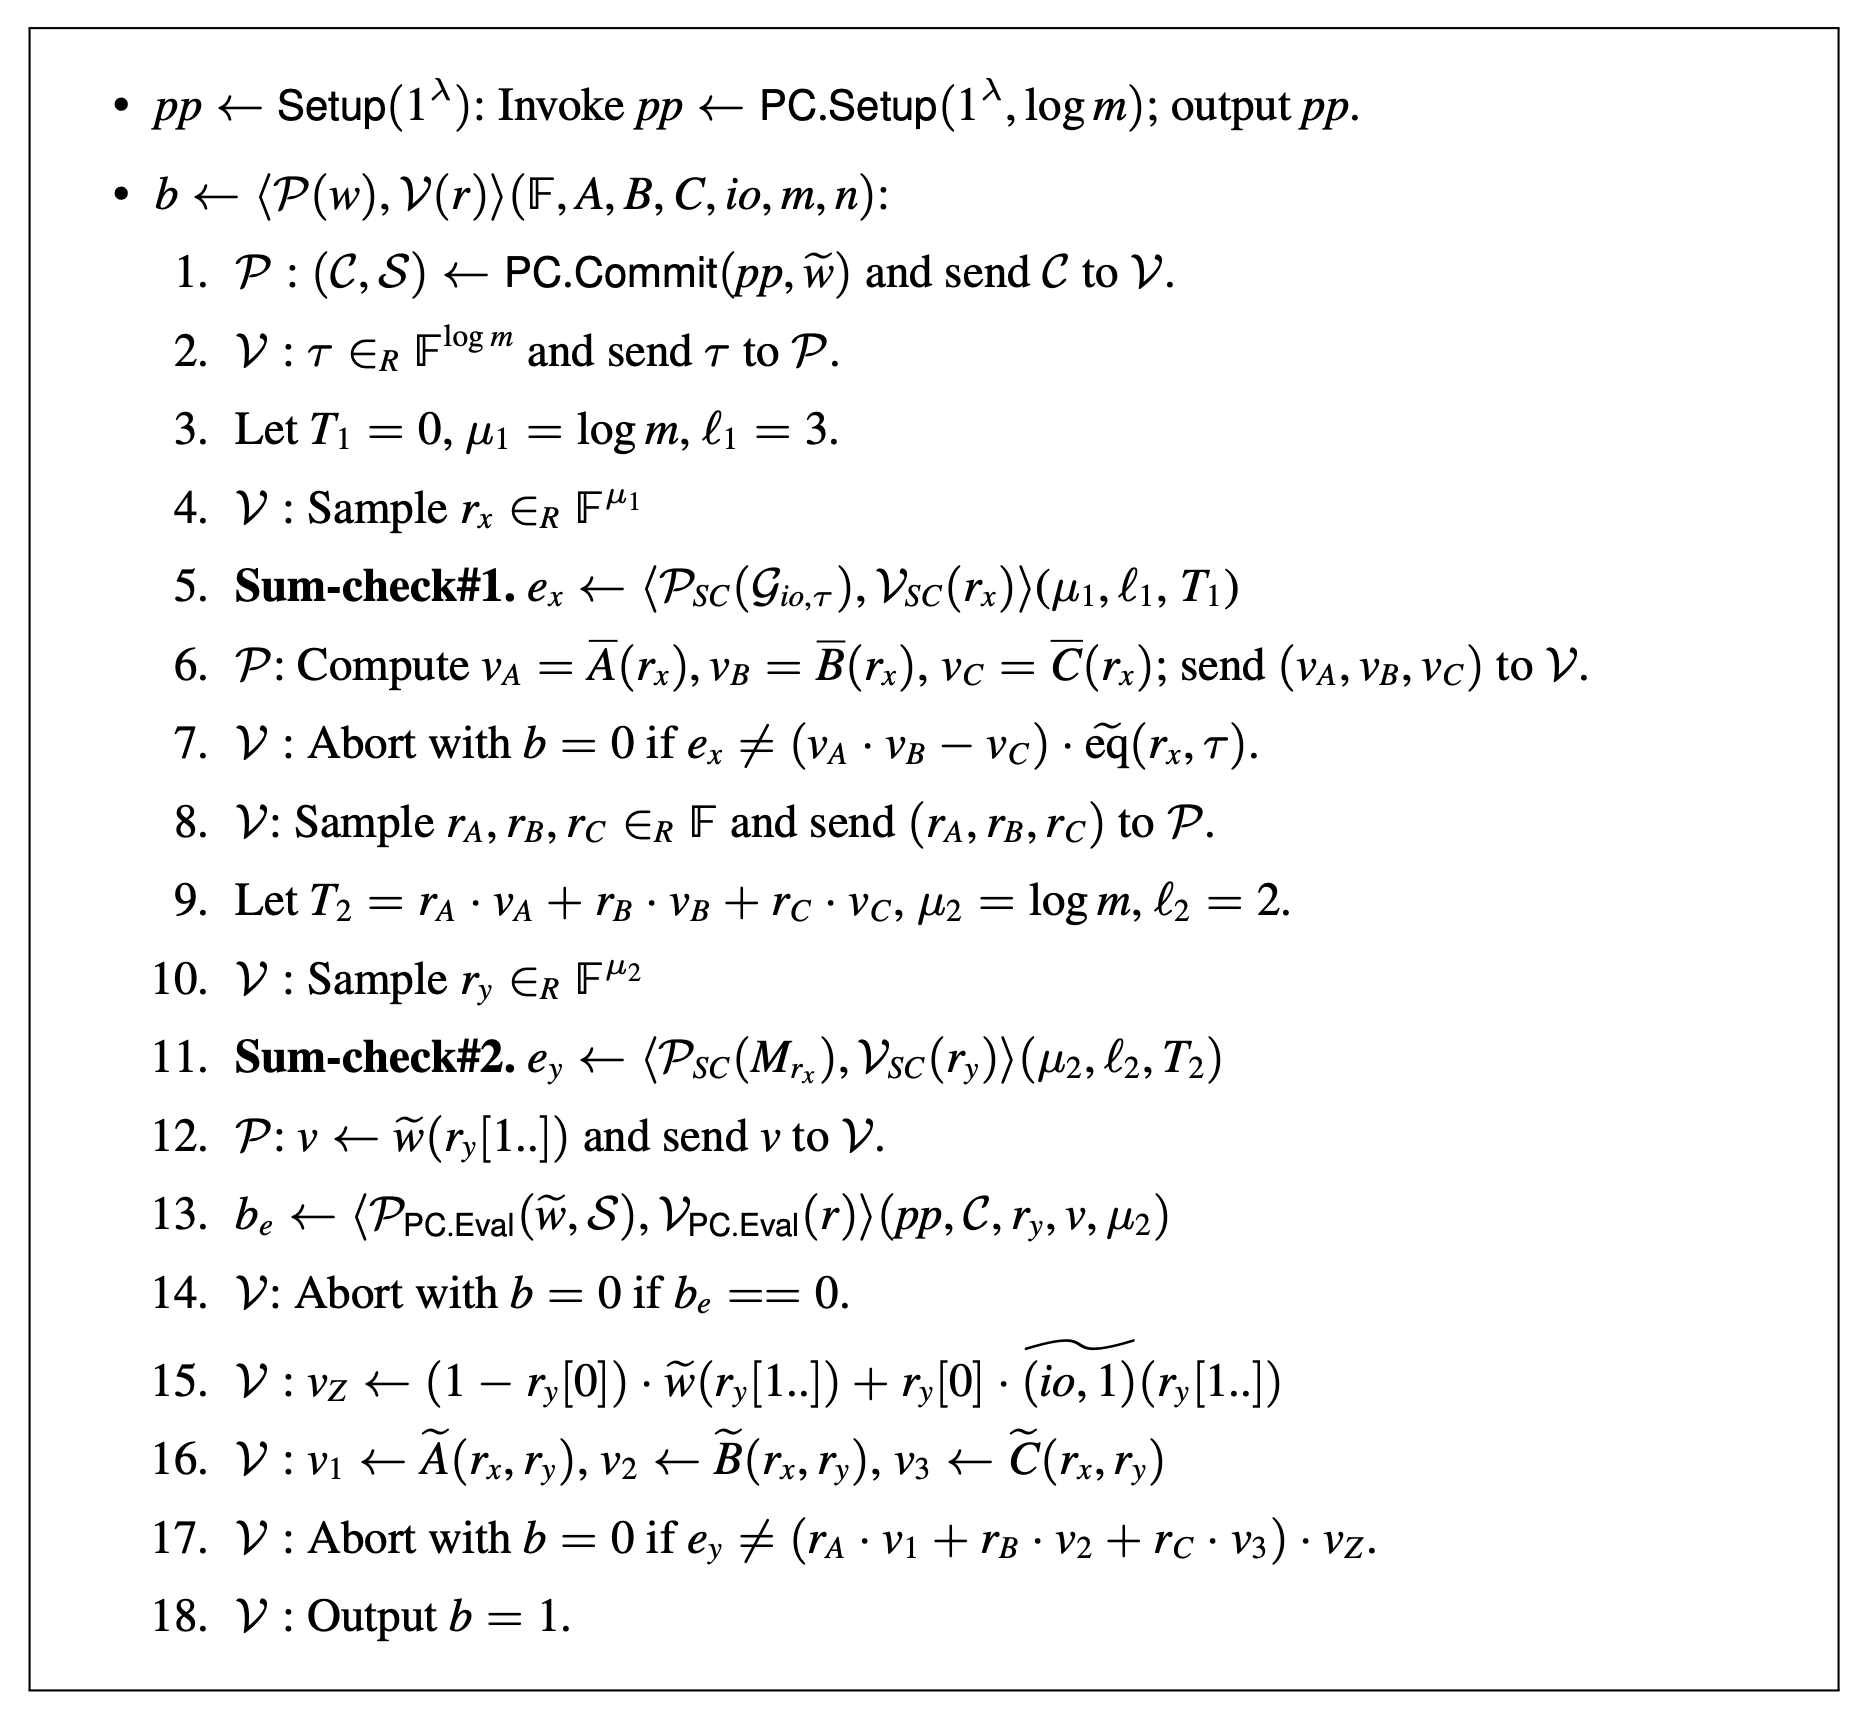
\includegraphics{figures/spartan-description.png}
    \caption{The Spartan protocol description, from the original paper.}
    \label{fig:spartan_protocol}
\end{figure}

After stripping away the polynomial commitment scheme, the protocol has the following structure:

\begin{description}
    \item[Setup:] This step is part of the polynomial commitment scheme and is not part of the PIOP we formalize.
    \item[Interaction:] The interaction is between a prover $\mathcal{P}$ with witness $w$ and a verifier $\mathcal{V}$ with public inputs $(\mathbb{F}, A, B, C, \text{io}, m, n)$.
    \begin{enumerate}
        \item $\mathcal{P}$: Sends oracle access to the multilinear extension of the witness, $\tilde{w}$, to $\mathcal{V}$. In the original paper, this is a commitment $(C,S) \leftarrow \text{PC.Commit}(\text{pp}, \tilde{w})$.
        \item $\mathcal{V}$: Samples a random challenge $\tau \in \mathbb{F}^{\log m}$ and sends it to $\mathcal{P}$.
        \item Let $T_1 = 0$, $\mu_1 = \log m$, $\ell_1 = 3$. These are parameters for the first sum-check protocol.
        \item $\mathcal{V}$: Samples a random challenge $r_x \in \mathbb{F}^{\mu_1}$.
        \item \textbf{Sum-check\#1.} A sum-check protocol is executed. The verifier receives the claimed evaluation $e_x$. The prover of the sum-check has oracle access to a polynomial $G_{io, \tau}$, and the verifier has oracle access to $r_x$. The parameters for this sub-protocol are $(\mu_1, \ell_1, T_1)$.
        \item $\mathcal{P}$: Computes evaluations $v_A = \tilde{A}(r_x)$, $v_B = \tilde{B}(r_x)$, $v_C = \tilde{C}(r_x)$ and sends them to $\mathcal{V}$. $\tilde{A}, \tilde{B}, \tilde{C}$ are multilinear extensions of the matrices $A, B, C$.
        \item $\mathcal{V}$: Aborts if $e_x \neq (v_A \cdot v_B - v_C) \cdot \tilde{\text{eq}}(r_x, \tau)$. This is the verifier's check for the first sum-check.
        \item $\mathcal{V}$: Samples random challenges $r_A, r_B, r_C \in \mathbb{F}$ and sends them to $\mathcal{P}$.
        \item Let $T_2 = r_A \cdot v_A + r_B \cdot v_B + r_C \cdot v_C$, $\mu_2 = \log n$, $\ell_2 = 2$. These are parameters for the second sum-check protocol. Note: The image states $\mu_2 = \log m$, which is likely a typo and should be $\log n$.
        \item $\mathcal{V}$: Samples a random challenge $r_y \in \mathbb{F}^{\mu_2}$.
        \item \textbf{Sum-check\#2.} Another sum-check protocol is executed. The verifier receives the claimed evaluation $e_y$.
        \item $\mathcal{P}$: Computes $v \leftarrow \tilde{w}(r_y[1..])$ and sends $v$ to $\mathcal{V}$.
        \item This step involves a polynomial commitment evaluation proof. In our PIOP formalization, this check is not needed as the verifier has direct oracle access to $\tilde{w}$.
        \item $\mathcal{V}$: This step is part of the evaluation proof check, so it is omitted.
        \item $\mathcal{V}$: Computes $v_Z \leftarrow (1 - r_y[0]) \cdot \tilde{w}(r_y[1..]) + r_y[0] \cdot \widetilde{(\text{io}, 1)}(r_y[1..])$. This reconstructs the evaluation of the combined input-witness vector polynomial $\tilde{z}$.
        \item $\mathcal{V}$: Queries oracles for $\tilde{A}, \tilde{B}, \tilde{C}$ at $(r_x, r_y)$ to get $v_1, v_2, v_3$.
        \item $\mathcal{V}$: Aborts if $e_y \neq (r_A \cdot v_1 + r_B \cdot v_2 + r_C \cdot v_3) \cdot v_Z$. This is the final check.
        \item $\mathcal{V}$: Outputs 1.
    \end{enumerate}
\end{description}

\subsection{Formalization using IOR Composition}


% Copyright (c) 2025 ZKLib Contributors. All rights reserved.
% Released under Apache 2.0 license as described in the file LICENSE.
% Authors: Poulami Das (Least Authority)

\section{Stir}

\subsection{Tools for Reed Solomon codes}
\subsubsection{Random linear combination as a proximity generator}\label{sec:proximity_gap}

\begin{theorem}\label{thm:proximity_gap}
\lean{proximity_gap}
\uses{def:distance_from_code,def:reed_solomon_code,def:list_close_codewords}
    Let $\code := \rscode[\field,\evaldomain,\degree]$ be a Reed Solomon code with rate $\rate:=\frac{\degree}{|\evaldomain|}$ and let $B^*(\rate):=\sqrt{\rate}$. For every $\distance \in (0,1 - B^*(\rate))$ and functions $f_0,\ldots,f_{m-1} : \evaldomain \to \field$, if
    \[
    \Pr_{r\leftarrow\field}\!\Bigl[
      \Delta\Bigl(\sum_{j=0}^{m-1} r^j\cdot {f_j},\rscode[\field,\evaldomain,\degree]\Bigr)
      \le \delta
    \Bigr]>\err^*(\degree,\rate,\distance,m),
    \]
    then there exists a subset $S \subseteq \evaldomain$ with $|S| \ge (1 - \delta)\cdot|L|$,
    and for every $i \in [m]$, there exists $u \in \rscode[\field,\evaldomain,\degree]$ such that $f_i(S) = u(S)$.
    
    \medskip
    
    \noindent
    Above, $\err^*(\degree,\rate,\distance,m)$ is defined as follows:
    \begin{itemize}
        \item if $\distance \in \left(0,\frac{1-\rate}{2}\right]$ then
            \[
                \err^*(\degree,\rate,\distance,m)=\frac{(m-1)\cdot \degree}{\rate\cdot|\field|}
            \]
        \item if $\distance \in \Bigl(\frac{1-\rate}{2}, 1-\sqrt{\rate}\Bigr)$ then
        \[
            \err^*(\degree,\rate,\distance,m)=\frac{(m-1)\cdot {\degree}^2}{|\field|\cdot{\Bigl(2\cdot\min\{1-\sqrt{\rate}-\distance,\frac{\sqrt{\rate}}{20}\}\Bigr)}^7}
        \]
    \end{itemize}
\end{theorem}

\subsubsection{Univariate Function Quotienting}\label{sec:quotienting}

In the following, we start by defining the \emph{quotient} of a univariate function.
\begin{definition}\label{def:quotient}
\lean{Quotienting.funcQuotient}
    Let $f:\evaldomain\to\field$ be a function, $S\subseteq\field$ be a set, and $\mathsf{Ans},\mathsf{Fill}: S\rightarrow\field$ be functions. Let $\hat{\mathsf{Ans}}\in\field^{<|S|}[X]$ be the (unique) polynomial with $\hat{\mathsf{Ans}}(x)=\mathsf{Ans}(x)$ for every $x\in S$, and let $\hat{V}_S\in\field^{<|S|+1}[X]$ be the unique non-zero polynomial with $\hat{V}_S(x)=0$ for every $x\in S$.
    The \emph{quotient function} $\mathsf{Quotient}\bigl(f,S,\mathsf{Ans},\mathsf{Fill}\bigr): \evaldomain\to\field$
    is defined as follows:
    \[
    \forall x \in \evaldomain,\quad
    \mathsf{Quotient}\bigl(f,S,\mathsf{Ans},\mathsf{Fill}\bigr)(x)  
    :=
    \begin{cases}
        \mathsf{Fill}(x)
        & \text{if } x \in S \\[6pt]
        \dfrac{f(x) - \hat{\mathsf{Ans}}(x)}{\hat{V}_S(x)}
        & \text{otherwise}
    \end{cases}
    \]
\end{definition}

Next we define the polynomial quotient operator, which quotients a polynomial relative to its output on evaluation points. The polynomial quotient is a polynomial of lower degree.

\begin{definition}\label{def:poly_quotient}
\lean{Quotienting.polyQuotient}
    Let $\hat{f}\in\field^{<\degree}[X]$ be a polynomial and $S\subseteq\field$ be a set, let $\hat{V}_S\in\field^{<|S|+1}[X]$ be the unique non-zero polynomial with $\hat{V}_S(x)=0$ for every $x\in S$. The \emph{polynomial quotient} $\mathsf{PolyQuotient}(\hat{f},S)\in\field^{<d-|S|}[X]$ is defined as follows:
    \[
            \mathsf{PolyQuotient}(\hat{f},S)(X):=\frac{\hat{f}(X)-\hat{\mathsf{Ans}}(X)}{\hat{V}_S(X)}
    \]
where $\hat{Ans}\in\field^{<|S|}[X]$ is the unique non-zero polynomial with $\hat{Ans}(x)=\hat{f}(x)$ for every $x \in S$.
\end{definition}

The following lemma, implicit in prior works, shows that if the function is ``quotiented by the wrong value'', then its quotient is far from low-degree.

\begin{lemma}\label{lemma:quotienting}
\lean{Quotienting.quotienting}
\uses{def:quotient,def:reed_solomon_code,def:distance_from_code,def:list_close_codewords}
    Let $f:\evaldomain\rightarrow\field$ be a function, $\degree\in\N$ be the degree parameter, $\distance\in(0,1)$
    be a distance parameter, $S\subseteq\field$ be a set with $|S|<\degree$, and $\mathsf{Ans},\mathsf{Fill}:S\rightarrow\field$ are functions. Suppose that for every $u\in\listcode(f,\degree,\distance)$ there exists $x\in S$ with $\hat{u}(x)\neq\mathsf{Ans}(x)$. Then 
    \[
            \Delta(\mathsf{Quotient}(f,S,\mathsf{Ans},\mathsf{Fill}),\rscode[\field,\evaldomain,\degree-|S|])+\frac{|T|}{|\evaldomain|}>\distance,
    \]
    where $T:=\{x\in\evaldomain\cap S: \hat{\mathsf{Ans}}(x)\neq f(x)\}$.
\end{lemma}

\subsubsection{Out of domain sampling}\label{sec:out_of_domain_smpl}
\begin{lemma}\label{lemma:out_of_domain_smpl}
\lean{OutOfDomSmpl.out_of_dom_smpl_1, OutOfDomSmpl.out_of_dom_smpl_2}
\uses{def:reed_solomon_code,def:list_decodable,def:list_close_codewords}
    Let $f:\evaldomain\rightarrow\field$ be a function, $\degree\in\N$ be a degree parameter, $s\in\N$ be a repetition parameter, and $\distance\in[0,1]$ be a distance parameter. If $\rscode[\field,\evaldomain,\degree]$ be $(\degree,l)$-list decodable then
    \begin{align*}
    \Pr_{r_1,\ldots,r_s\gets\field\setminus\evaldomain}[\exists\text{ distinct }u,u'\in\listcode(f,\degree,\distance):\forall i\in[s],\hat{u}(r_i)=\hat{u}'(r_i)] & \leq \binom{l}{2}\cdot{\Big(\frac{\degree-1}{|\field|-|\evaldomain|}\Big)}^s \\
    & \leq \Big(\frac{l^2}{2}\Big)\cdot{\Big(\frac{\degree}{|\field|-|\evaldomain|}\Big)}^s
    \end{align*}
\end{lemma}

\subsubsection{Folding univariate functions}\label{sec:folding_uf}
STIR relies on $k$-wise folding of functions and polynomials - this is similar to prior works, although presented in a slightly different form. As shown below, folding a function preserves proximity from the Reed-Solomon code with high probability. The folding operator is based on the following fact, decomposing univariate polynomials into bivariate ones.

\begin{lemma}\label{fact:poly_folding} 
\lean{Folding.exists_unique_bivariate,Folding.degree_bound_bivariate}
Given a polynomial $\hat{q}\in\field[X]$:
\begin{itemize}
        \item For every univariate polynomial $\hat{f}\in\field[X]$, there exists a unique bivariate polynomial $\hat{Q}\in\field[X,Y]$ with:
        \[
          \polydeg_X(\hat{Q}) := \left\lfloor \frac{\polydeg(\hat{f})}{\polydeg(\hat{q})} \right\rfloor,\quad \polydeg_Y(\hat{Q}) < \polydeg(\hat{q})
        \]
        such that $\hat{f}(Z)=\hat{Q}(\hat{q}(Z),Z)$. Moreover, $\hat{Q}$ can be computed efficiently given $\hat{f}$ and $\hat{q}$. Observe that if $\polydeg(\hat{f})<t\cdot\polydeg(\hat{q})$ then
        $\polydeg(\hat{Q})<t$.
        
        \item For every $\hat{Q}[X,Y]$ with $\polydeg_X(\hat{Q})<t$ and $\polydeg_Y(\hat{Q})<\polydeg(\hat{q})$, the polynomial $\hat{f}(Z)=\hat{Q}(\hat{q}(Z),Z)$ has degree $\polydeg(\hat{f})<t\cdot\polydeg(\hat{q})$.
\end{itemize}
\end{lemma}

Below, we define folding of a polynomial followed by folding of a function.
\begin{definition}\label{def:poly_folding}
\lean{Folding.polyFold}
\uses{fact:poly_folding}
    Given a polynomial $\hat{f}\in\field^{<\degree}[X]$, a folding parameter $k\in\N$ and $r\in\field$, we define a polynomial $\mathsf{PolyFold}(\hat{f},k,r)\in\field^{\degree/k}[X]$ as follows. Let $\hat{Q}[X,Y]$ be the bivariate polynomial derived from $\hat{f}$ using Fact~\ref{fact:poly_folding} with $\hat{q}(X):=X^k$. Then $\mathsf{PolyFold}(\hat{f},k,r)(X):=\hat{Q}(X,r)$.
\end{definition}

\begin{definition}\label{def:fn_folding}
\lean{Folding.fold}
Let $f:\evaldomain\rightarrow\field$ be a function, $k\in\N$ a folding parameter and $\alpha\in\field$. For every $x\in{\evaldomain}^k$, let $\hat{p}_x\in\field^{<k}[X]$ be the polynomial where $\hat{p}_x(y)=f(y)$ for every $y\in{\evaldomain}$ such that $y^k=x$. We define $\mathsf{Fold}(f,k,\alpha):\evaldomain\rightarrow\field$ as follows.
\[
    \mathsf{Fold}(f,k,\alpha):=\hat{p}_x(\alpha).
\]
In order to compute $\mathsf{Fold}(f,k,\alpha)(x)$ it suffices to interpolate the $k$ values $\{f(y):y\in\evaldomain\text{ s.t. }y^k=x\}$ into the polynomial $\hat{p}_x$ and evaluate this polynomial at $\alpha$.
\end{definition}

The following lemma shows that the distance of a function is preserved under folding. If a functions $f$ has distance $\distance$ to a Reed-Solomon code then, with high probability over the choice of folding randomness, its folding also has a distance of $\distance$ to the ``$k$-wise folded'' Reed-Solomon code.

\begin{lemma}\label{lemma:folding}
\lean{Folding.folding}
\uses{def:reed_solomon_code,def:fn_folding,def:distance_from_code}
    For every function $f:\evaldomain\rightarrow\field$, degree parameter $\degree\in\N$, folding parameter $k\in\N$, distance parameter $\distance\in(0,\min\{{\Delta(\mathsf{Fold}[f,k,r^{\mathsf{fold}}],\rscode[\field,{\evaldomain}^k, \degree/k]),1-{\mathsf{B}}^*(\rate)}\})$, letting $\rate:=\frac{\degree}{|\evaldomain|}$,
    \[
        \Pr_{r^{\mathsf{fold}}\gets\field}[\Delta(\mathsf{Fold}[f,k,r^{\mathsf{fold}}],\rscode[\field,{\evaldomain}^k, \degree/k])<\distance]>\err^*(\degree/k,\rate,\distance,k).
    \]
    Above, ${\mathsf{B}}^*$ and ${\err}^*$ are the proximity bound and error (respectively) described in Section~\ref{sec:proximity_gap}.
\end{lemma}

\subsubsection{Combine functions of varying degrees}\label{sec:combine}
We show a new method for combining functions of varying degrees with minimal proximity require- ments using geometric sums. We begin by recalling a fact about geometric sums.

\begin{lemma}\label{fact:geometric_sum}
\lean{Combine.geometric_sum_units}
    Let $\field$ be a field, $r\in\field$ be a field element, $a\in\N$ be a natural number. Then
    \[
        \sum_{i=0}^{a}r^i:=
        \begin{cases}
        \Big(\frac{1-r^{a+1}}{1-r}\Big) & r\neq 1 \\
        a+1 & r=1
        \end{cases}
    \]
\end{lemma}

\begin{definition}\label{def:combine}
\lean{Combine.combineInterm,Combine.combineFinal}
    Given target degree $\degree^*\in\N$, shifting parameter $r\in\field$, functions $f_0,\ldots,f_{m-1}:\evaldomain\rightarrow\field$, and degrees $0\leq \degree_0,\ldots,\degree_{m-1}\leq {\degree}^*$, we define $\combine(\degree^*,r,(f_0,\degree_0),\ldots,(f_{m-1},\degree_{m-1})):\evaldomain\rightarrow\field$ as follows:
    \begin{align*}
        \combine({\degree}^*,r,(f_0,\degree_0),\ldots,(f_{m-1},\degree_{m-1}))(x)&:=\sum_{i=0}^{m-1}r_i\cdot f_i(x)\cdot \Big(\sum_{l=0}^{\degree^*-\degree_i}{(r\cdot x)}^l\Big) \\
        &= 
        \begin{cases}
            \sum_{i=0}^{m-1}r_i\cdot f_i(x)\cdot \Big(\frac{1-{(xr)}^{\degree^*-\degree_i+1}}{1-xr}\Big) & x\cdot r\neq 1\\
            \sum_{i=0}^{m-1}r_i\cdot f_i(x)\cdot (\degree^*-\degree_i+1) & x\cdot r= 1
        \end{cases}
    \end{align*}
Above, $r_i:=r^{i-1+\sum_{j<i}(\degree^*-\degree_j)}$.
\end{definition}

\begin{definition}\label{def:deg_corr}
\lean{Combine.degreeCorrInterm,Combine.degreeCorrFinal}
\uses{def:combine,def:reed_solomon_code,def:distance_from_code}
    Given target degree $\degree^*\in\N$, shifting parameter $r\in\field$, function $f:\evaldomain\rightarrow\field$, and degree $0\leq\degree\leq\degree^*$, we define $\degcorr(\degree^*,r,f,\degree)$ as follows.
    \[
        \degcorr(\degree^*,r,f,\degree)(x):=f(x)\cdot\Bigg(\sum_{l=0}^{\degree^*-\degree}{(r\cdot x)}^l\Bigg)=
        \begin{cases}
            f(x)\cdot\frac{1-{(xr)}^{\degree^*-\degree_i+1}}{1-xr} & x\cdot r\neq 1\\
            f(x)\cdot (\degree^*-\degree_i+1) & x\cdot r = 1
        \end{cases}
    \]
(Observe that $\degcorr(\degree^*,r,f,\degree)=\combine(\degree^*,r,(f,\degree))$.)
\end{definition}

Below it is shown that combining multiple polynomials of varying degrees can be done as long as the proximity error is bounded by $(\min{\{1-{\mathsf{B}}^*(\rate),1-\rate-1/|\evaldomain|\}})$.

\begin{lemma}\label{lemma:combine}
\lean{Combine.combine}
\uses{def:reed_solomon_code,def:combine,def:deg_corr,thm:proximity_gap}
    Let $\degree^*$ be a target degree, $f_0,\ldots,f_{m-1}:\evaldomain\rightarrow\field$ be functions, $0\leq \degree_0,\ldots,\degree_{m-1}\leq \degree^*$ be degrees, $\distance\in\min{\{1-{\mathsf{B}}^*(\rate),1-\rate-1/|\evaldomain|\}}$ be a distance parameter, where $\rate=\degree^*/|\evaldomain|$. If
    \[
        \Pr_{r\gets\field}[\Delta(\combine(\degree^*,r,(f_0,\degree_0),\ldots,(f_{m-1},\degree_{m-1})),\rscode[\field,\evaldomain,\degree^*])]>\err^*(\degree^*,\rate,\distance,m\cdot(\degree^*+1)-\sum_{i=0}^{m-1}\degree_i),
    \] 
    then there exists $S\subseteq \evaldomain$ with $|S|\geq(1-\distance)\cdot|\evaldomain|$, and
    \[
        \forall i\in[m-1],\exists u\in\rscode[\field,\evaldomain,\degree_i], f_i(S)=u(S).
    \]
    Note that this implies $\Delta(f_i,\rscode[\field,\evaldomain,\degree_i])<\distance$ for every $i$. Above, ${\mathsf{B}}^*$ and ${\err}^*$ are the proximity bound and error (respectively) described in Section~\ref{sec:proximity_gap}.
\end{lemma}

\subsection{Stir Main theorems}

\begin{theorem}[STIR Main Theorem]\label{thm:stir}
\lean{StirIOP.stir_main}
\uses{def:reed_solomon_code,lemma:rnd_by_rnd_soundness}
    Consider the following ingrediants:
    \begin{itemize}
        \item A security parameter $\lambda\in\N$.
        \item A Reed-Solomon code $\rscode[\field,\evaldomain,\degree]$ with $\rate:=\frac{\degree}{|\evaldomain|}$ where $\degree$ is a power of $2$, and $\evaldomain$ is a smooth domain.
        \item A proximity parameter $\distance\in(0,1-1.05\cdot\sqrt{\rate})$.
        \item A folding parameter $k\in\N$ that is power of $2$ with $k\geq 4$.
    \end{itemize}
If $|\field|=\Omega(\frac{\lambda\cdot2^\lambda\cdot\degree^2\cdot{|\evaldomain|}^2}{\log(1/\rate)})$, there is a public-coin IOPP for $\rscode[\field,\evaldomain,\degree]$ with the following parameters:
\begin{itemize}
    \item Round-by-round soundness error $2^{-\lambda}$.
    \item Round complexity: $M:=O(\log_k{\degree})$.
    \item Proof length: $|\evaldomain|+O_k(\log{\degree})$.
    \item Query complexity to the input: $\frac{\lambda}{-\log{(1-\distance)}}$.
    \item Query complexity to the proof strings: $O_k(\log{\degree}+\lambda\cdot\log{\Big(\frac{\log{\degree}}{\log{1/\rate}}\Big)})$.
\end{itemize}
\end{theorem}

\begin{lemma}\label{lemma:rnd_by_rnd_soundness}
\lean{StirIOP.stir_rbr_soundness}
\uses{def:reed_solomon_code,def:list_decodable,lemma:folding,lemma:out_of_domain_smpl,lemma:quotienting,lemma:combine}
    Consider $(\field,M,\degree,k_0,\ldots,k_M,\evaldomain_0,\ldots,\evaldomain_M,t_0,\ldots,t_M)$ and for every $i\in\{0,\ldots,M\}$, let $\degree_i:=\frac{\degree}{\prod_{j<i}k^j}$ and $\rate_i:=\degree_i/|\evaldomain_i|$. For every $f\notin\rscode[\field,\evaldomain_0,\degree_0]$ and every $\distance_0,\ldots,\distance_M$ where
    \begin{itemize}
        \item $\distance_0\in(0,\Delta(f,\rscode[\field,\evaldomain_0,\degree_0])]\cap(0,1-{\mathsf{B}}^*(\rate_0))$
        \item for every $0<i\leq M$: $\distance_i\in(0,\min{\{1-\rate_i-\frac{1}{|\evaldomain_i|},1-{\mathsf{B}^*(\rate_i)}\}})$, and
        \item for every $0<i\leq M$: $\rscode[\field,\evaldomain_i,\degree_i]$ is $(\distance_i,l_i)$-list decodable,
    \end{itemize}
    There exists an IOPP with above parameters, that has round-by-round soundness error $(\epsilon^{\mathsf{fold}},\epsilon^{\mathsf{out}}_1,\epsilon^{\mathsf{shift}}_1,\ldots,\epsilon^{\mathsf{out}}_M,\epsilon^{\mathsf{shift}}_M,\epsilon^{\mathsf{fin}})$ where:
    \begin{itemize}
        \item $\epsilon^{\mathsf{fold}}\leq\err^*(\degree_0/k_0,\rate_0,\distance_0,k_0)$.
        \item $\epsilon^{\mathsf{out}}_i\leq\frac{l^2_i}{2}\cdot{\big(\frac{\degree_i}{|\field|-|\evaldomain_i|}\big)}^s$
        \item $\epsilon^{\mathsf{shift}}_i\leq {(1-\distance_{i-1})}^{t_{i-1}}+\err^*(\degree_i,\rate_i,\distance_i,t_{i-1}+s)+\err^*(\degree_i/k_i,\rate_i,\distance_i,k_i)$.
        \item $\epsilon^{\mathsf{fin}}\leq{(1-\distance_M)}^{t_M}$.
    \end{itemize}
    Above, ${\mathsf{B}}^*$ and ${\err}^*$ are the proximity bound and error (respectively) described in Section~\ref{sec:proximity_gap}.
\end{lemma}



% Copyright (c) 2025 ZKLib Contributors. All rights reserved.
% Released under Apache 2.0 license as described in the file LICENSE.
% Authors: Poulami Das (Least Authority)

\section{Whir}

\subsection{Tools for Reed Solomon codes}

\subsubsection{Mutual Correlated Agreement as a Proximity Generator}

\begin{definition}\label{def:proximity_generator}
\lean{Generator.ProximityGenerator}
\uses{def:linear_code,def:distance_from_code}
Let $\code\subseteq \field^{\evaldomain}$ be a linear code. We say that $\mathsf{Gen}$ is a proximity generator for $\code$ with proximity bounds ${\bound}$ and $\err$ if the following implication holds for $f_0,\ldots,f_{\parl-1} : \evaldomain \rightarrow \field$ and $\delta\in(0,1-{\bound}(\rate,\parl))$. If
\begin{align*}
    \Pr_{r_0,\ldots,r_{\parl-1}\leftarrow \gen}[\Delta(\sum_{i\in[0,(\parl-1)]} r_i \cdot f_i, \code) \le \delta] > err(\code,\parl,\delta),
\end{align*}
then there exists $S\subseteq \evaldomain$, $|S|>(1-\delta)\cdot|\evaldomain|$, and
$\forall i \in [0, (\parl-1)]$, $\exists u \in \code, \forall x \in S$, $f_i(x)=u(x)$. 
\end{definition}

\begin{theorem}\label{thm:proximity_gap_whir}
\lean{RSGenerator.proximityGapTheorem}
\uses{def:proximity_generator,def:reed_solomon_code}
    Let $\code = \rscode[\field,\evaldomain,m]$ be a Reed Solomon code with rate $\rate = 2^m/|\evaldomain|$. $\gen(\alpha,\parl)=\{1,\alpha,\ldots,\alpha^{\parl-1}\}$ is a proximity generator for $\code$ with proximity bounds ${\bound}(\rate,\parl)=\sqrt{\rate}$ and $\err(C,\parl,\delta)$ defined below.
    \begin{itemize}
        \item if $\distance \in \left(0,\frac{1-\rate}{2}\right]$ then
            \[
                \err(\code,\parl,\delta)=\frac{(m-1)\cdot \degree}{\rate\cdot|\field|}
            \]
        \item if $\distance \in \Bigl(\frac{1-\rate}{2}, 1-\sqrt{\rate}\Bigr)$ then
        \[
            \err(\code,\parl,\delta)=\frac{(m-1)\cdot {\degree}^2}{|\field|\cdot{\Bigl(2\cdot\min\{1-\sqrt{\rate}-\distance,\frac{\sqrt{\rate}}{20}\}\Bigr)}^7}
        \]
    \end{itemize}
\end{theorem}

\begin{definition}\label{def:gen_mutual_corr_agreement}
    \lean{CorrelatedAgreement.genMutualCorrAgreement}
    \uses{def:proximity_generator}
    Let $\code$ be a linear code. We say that $\gen$ be a proximity generator with mutual correlated agreement with proximity bounds ${\bound}^\star$ and $\err^\star$, if for $f_0,\ldots,f_{\parl-1}:\evaldomain\rightarrow\field$ and $\delta\in(0,1-{\bound}^\star(\code,\parl))$ the following holds.
    \[
    \Pr_{(r_0, \ldots, r_{\parl-1}) \leftarrow \gen(\parl)} \left[
        \exists S \subseteq \evaldomain \;\; s.t.\;\;
        \begin{array}{l}
        |S| \geq (1 - \delta) \cdot |\evaldomain| \\
        \land\; \exists u \in \code, u(S) = \sum_{j \in [0,(\parl-1)]} r_j \cdot f_j(S) \\
        \land\; \exists i \in [0,(\parl-1)], \forall u' \in \code, u'(S) \neq f_i(S)
        \end{array}\right]
    \leq \err^\star(\code, \parl, \delta).
    \]
\end{definition}

\begin{lemma}\label{lemma:gen_mutual_corr_agreement}
\lean{CorrelatedAgreement.genMutualCorrAgreement_le_bound}
\uses{def:proximity_generator, def:gen_mutual_corr_agreement}
    Let $\code$ be a linear code with minimum distance $\delta_{\code}$ and let $\gen$ be a proximity generator for $\code$ with proximity bound ${\bound}$ and error $\err$. Then $\gen$ has mutual correlated agreement with proximity bound ${\bound}^\star(\code, \parl) = \min\{1 - \delta_{\code}/2, \bound(\code, \parl)\}$ and error $\err^\star(\code, \parl, \delta) := \err(\code, \parl, \delta)$.
\end{lemma}

\begin{lemma}
\lean{CorrelatedAgreement.genMutualCorrAgreement_rsc_le_bound}
\uses{lemma:gen_mutual_corr_agreement, def:reed_solomon_code}
    Let $\code := \rscode[\field, \evaldomain, m]$ be a Reed Solomon code with rate $\rate$. The function $\gen(\parl; \alpha) = (1, \alpha, \ldots, \alpha^{\parl - 1})$ is a proximity generator for $\code$ with mutual correlated agreement with proximity bound ${\bound}^\star(\code, \parl) := \frac{1 + \rate}{2}$ and error $\err^\star(\code, \parl, \delta) = \frac{(\parl - 1) \cdot 2^m}{\rate \cdot |\field|}$.
\end{lemma}

\begin{theorem}\label{conjecture:whir}
\lean{CorrelatedAgreement.genMutualCorrAgreement_le_johnsonBound,CorrelatedAgreement.genMutualCorrAgreement_le_capacity}
\uses{def:reed_solomon_code,lemma:gen_mutual_corr_agreement}
    The function $\gen(\parl; \alpha) := (1, \alpha, \ldots, \alpha^{\parl - 1})$ is a proximity generator with mutual correlated agreement for every smooth Reed Solomon code $\code := \rscode[\field, \evaldomain, m]$ (with rate $\rate := 2^m / |\evaldomain|$). We give two conjectures, for the parameters of the proximity bound ${\bound}^\star$ and the error $\err^\star$:
    \begin{enumerate}
        \item \textit{Up to the Johnson bound:} ${\bound}^\star(\code, \parl) := \sqrt{\rate},$ \textit{and}
        \[
        \err(\code, \parl, \delta) := \frac{(\parl - 1) \cdot 2^m}{|\field| \cdot \left( 2 \cdot \min\left\{1 - \sqrt{\rate} - \delta, \frac{\sqrt{\rate}}{20} \right\} \right)^7}.
        \]
      
        \item \textit{Up to capacity:} ${\bound}^\star(\code, \parl) := \rate$, \textit{and there exist constants $c_1, c_2, c_3 \in \mathbb{N}$ such that for every $\eta > 0$ and $0 < \delta < 1 - \rate - \eta$:}
        \[
        \err^\star(\code, \parl, \delta) := \frac{(\parl - 1)^{c_2} \cdot \delta^{c_2}}{\eta^{c_1} \cdot \rate^{c_1 + c_2} \cdot |\field|}.
        \]
      \end{enumerate}
\end{theorem}

\subsubsection{Mutual correlated agreement preserves list decoding}

\begin{lemma}\label{lemma: mutual_corrAgr_listdecoding}
\lean{CorrelatedAgreement.mutualCorrAgreement_list_decoding}
\uses{def:reed_solomon_code,def:interleaved_code,def:list_close_codewords,lemma:gen_mutual_corr_agreement}
    Let $\code \subseteq \field^{\evaldomain}$ be a linear code with minimum distance $\delta_{\code}$, and let $\gen$ be a proximity generator for $\code$ with mutual correlated agreement with proximity bound ${\bound}^\star$ and error $\err^\star$. Then, for every $f_0, \ldots, f_{\parl-1} : \evaldomain \to \field$ and $\delta \in (0, \min\{\delta_{\code}, 1 - {\bound}^\star(\code, \parl)\})$:
    \[
    \Pr_{\substack{\alpha \leftarrow \{0,1\}^{w^\star} \\ \boldsymbol{r} := \gen(\parl; \alpha)}} \left[
    \Lambda\left(\code, \sum_{j \in [0,(\parl-1)]} r_j \cdot f_j, \delta \right) \neq 
    \left\{ \sum_{j \in [0,(\parl-1)]} r_j \cdot u_j : \boldsymbol{u} \in \Lambda\left(\mathcal{C}^\ell, (f_0, \ldots, f_{\parl-1}), \delta \right) \right\}
    \right] \leq \err^\star(\code, \parl, \delta).
    \]
\end{lemma}

\subsubsection{Folding univariate functions}

\begin{definition}\label{def:extract}
\lean{Fold.extract_x}
    Let $\mathsf{extract}:\evaldomain^{2^{k+1}}\rightarrow \evaldomain^{2^k}$ be a function. There exists $x \in \evaldomain$, such that $y = x^{2^{k+1}}\in\evaldomain^{2^{k+1}}$. Then $\mathsf{extract}$ returns $z = \sqrt{y} = x^{2^k}\in\evaldomain^{2^k}$ such that $y = z^2$.
\end{definition}

\begin{definition}\label{def:foldf}
\lean{Fold.foldf}
\uses{def:extract}
    Let $f : \evaldomain^{2^k} \to \field$ be a function, and $\alpha \in \field$. We define $\mathrm{Fold_f}(f, {\alpha}) : \evaldomain^{(2^{k+1})} \to \field$ as follows:
    \[
    \forall x \in \evaldomain^{2^k}, y \in \evaldomain^{2^{k+1}}, \quad \mathrm{Fold_f}(f, \alpha)(y) := \frac{f(x) + f(-x)}{2} + \alpha \cdot \frac{f(x) - f(-x)}{2 \cdot x}.
    \]

    In order to compute $\mathrm{Fold_f}(f, \alpha)(y)$ it suffices to query $f$ at $x$ and $-x$, by retrieving $x=\mathsf{extract}(y)$.
\end{definition}

\begin{definition}\label{def:fold_k}
\lean{Fold.fold_k_core,Fold.fold_k}
\uses{def:foldf}
    For $k \leq m$ and $\vec{\alpha} = (\alpha_0, \ldots, \alpha_{k-1}) \in \field^k$ we define $\mathrm{Fold}(f, \vec{\alpha}) : \evaldomain^{2^k} \to \field$ to equal $\mathrm{Fold}(f, \vec{\alpha}) := f_k$ where $f_k$ is defined recursively as follows: $f_0 := f$, and $f_i := \mathrm{Fold_f}(f_{i-1}, \alpha_i)$. 
\end{definition}

\begin{definition}\label{def:fold_k_set}
\lean{Fold.fold_k_set}
\uses{def:fold_k}
    For a set $S \subseteq \field^{\evaldomain}$ we denote $\mathrm{Fold_{S}}(S, \vec{\alpha}) := \{\mathrm{Fold_{S}}(f, \vec{\alpha}) \mid f \in S\}$.
\end{definition}

\begin{lemma}\label{lemma:fold_fg}
\lean{Fold.fold_f_g}
\uses{def:fold_k,def:smooth_rs_code}
    Let $f : \evaldomain \to \field$ be a function, $\vec{\alpha} \in \field^k$ folding randomness and let $g := \mathrm{Fold}(f, \vec{\alpha})$. If $f \in \rscode[\field, \evaldomain, m]$ and $k \leq m$, then $g \in \rscode[\field, \evaldomain^{2^k}, m - k]$, and further the multilinear extension of $g$ is given by $\hat{g}(X_k, \ldots, X_{m-1}) := \hat{f}(\vec{\alpha}, X_k, \ldots, X_{m-1})$ where $\hat{f}$ is the multilinear extension of $f$.
\end{lemma}

\subsubsection{Block relative distance}

\begin{definition}\label{def:block}
    \lean{BlockRelDistance.block}
    Let $\evaldomain \subseteq \field$ be a smooth evaluation domain and $k \in \mathbb{N}$ be a folding parameter. For $z \in \evaldomain^{2^k}$, define $\mathrm{Block}(\evaldomain, i, k, z) := \{ x \in \evaldomain, y \in \evaldomain^{2^i} : y^{2^{k-i}} = z \}$.
\end{definition}

\begin{definition}\label{def:block_rel_distance}
\lean{BlockRelDistance.blockRelDistance}
\uses{def:block}
    Let $\code := \rscode[\field, \evaldomain, m]$ be a smooth Reed Solomon code and let $f, g : \evaldomain^{2^i} \to \field$. We define the $(i,k)$-wise block relative distance as
    \[
    \Delta_{r}(\code, i, k, f, g) = \frac{ \left| \left\{ z \in \evaldomain^{2^k} : \exists y \in \mathrm{Block}(\evaldomain, i, k, z), f(y) \neq g(y) \right\} \right| }{ |\evaldomain^{2^k}| }
    \]
\end{definition}

\begin{definition}\label{def:min_block_rel_distance}
\lean{BlockRelDistance.minBlockRelDistance}
\uses{def:block_rel_distance}
    For $S \subseteq \field^{\evaldomain}$, we let $\Delta_{r}(\code, i, k, f, S) := \min_{g \in S} \Delta_{r}(\code, i, k, f, g)$.
\end{definition}

{Note that $\Delta_{r}(\code, 0, 0, f, g) = \Delta(f, g)$ for any $\code$. We define the block list decoding of a codeword.}

\begin{definition}\label{def:list_close_codewords_block}
\lean{BlockRelDistance.listBlockRelDistance}
\uses{def:block_rel_distance}
    For a smooth Reed Solomon code $\rscode := \rscode[\field, \evaldomain, m]$, proximity parameter $\delta \in [0,1]$, and $f : \evaldomain^{2^i} \to \field$, we let
    \[
    \Lambda_{r}(\code, i, k, f, \delta) := \{ u \in \code \mid \Delta_{r}(\code, i, k, f, u) \leq \delta \},
    \]
    denote the list of codewords in $\code$ within relative block distance at most $\delta$ from $f$.
\end{definition}

\begin{lemma}\label{lemma:block_rel_distance}
\lean{BlockRelDistance.blockRelDistance_le_hammingDistance}
\uses{def:block_rel_distance,def:distance_from_code,def:list_close_codewords_block,def:list_close_codewords}
    For any $\code := \rscode[\field, \evaldomain, m]$, $k \in \mathbb{N}$, and $f, g : \evaldomain^{2^i} \to \field$, we have that $\Delta(f, g) \leq \Delta_{r}(\code, i, k, f, g)$. Consequently, $\Lambda_{r}(\code, i, k, f, \delta) \subseteq \Lambda(\code, f, \delta)$ for $\delta\in[0,1]$.
\end{lemma}

\subsubsection{Folding preserves list decoding}

\begin{theorem}\label{thm:folding_preserves_listdecoding}
\lean{Fold.folding_listdecoding_if_genMutualCorrAgreement}
\uses{lemma:folding_preserves_listdecoding_base, lemma:folding_preserves_listdecoding_bound, lemma:folding_preserves_listdecoding_base_ne_subset}
    Let $\code = \rscode[\field, \evaldomain, m]$ be a smooth Reed Solomon code and $k \leq m$. For $0 \leq i \leq k$ let $\code^{(i)} := \rscode[\field, \evaldomain^{2^i}, m - i]$. Let $\gen(\parl; \alpha) = (1, \alpha, \ldots, \alpha^{\parl - 1})$ be a proximity generator with mutual correlated agreement for the codes $\code^{(0)}, \ldots, \mathcal{C}^{(k-1)}$ with proximity bound ${\bound}^\star$ and error $\err^\star$. Then for every $f : \evaldomain \to \field$ and $\delta \in \left(0, 1 - \max_{i \in [0,(k-1)]} \{ {\bound}^\star(\code^{(i)}, 2) \} \right)$,
    \[
    \Pr_{\alpha \leftarrow \field^k} \left[
    \mathrm{Fold_S}(\Lambda_{r}(\code, 0, k, f, \delta), \alpha)
    \neq \Lambda(\code^{(k)}, \mathrm{Fold}(f, \alpha), \delta)
    \right] < \err^{(k)}(\code, \delta).
    \]
\end{theorem}

\begin{lemma}\label{lemma:folding_preserves_listdecoding_base}
\lean{Fold.folding_preserves_listdecoding_base}
\uses{def:list_close_codewords_block,def:fold_k,def:fold_k_set}
    Let $\code := \rscode[\field, \evaldomain, m]$ be a Reed Solomon code, and $k \leq m$ be a parameter. Denote $\code' := \rscode[\field, \evaldomain^{2}, m - 1]$. Then for every $f : \evaldomain \to \field$ and $\delta \in (0, 1 - {\bound}^\star(\code', 2))$,
    \[
    \Pr_{\alpha \leftarrow \field} \left[
    \mathrm{Fold_S}(\Lambda_{r}(\code, 0, k, f, \delta), \alpha)
    \neq \Lambda_{r}(\code', 1, k, \mathrm{Fold}(f, \alpha), \delta)
    \right] < \err^\star(\code', 2, \delta).
    \]
\end{lemma}
    
\begin{lemma}\label{lemma:folding_preserves_listdecoding_bound}
\lean{Fold.folding_preserves_listdecoding_bound}
\uses{def:list_close_codewords_block,def:fold_k}
    For every $\alpha \in \field$, $\mathrm{Fold_S}(\Lambda_{r}(\code, 0, k, f, \delta), \alpha) \subseteq \Lambda_{r}(\code', 1, k, \mathrm{Fold}(f, \alpha), \delta)$.
\end{lemma}

\begin{lemma}\label{lemma:folding_preserves_listdecoding_base_ne_subset}
\lean{Fold.folding_preserves_listdecoding_base_ne_subset}
\uses{def:list_close_codewords_block,def:fold_k,def:fold_k_set}
    \[
    \Pr_{\alpha \leftarrow \field} \left[
    \Lambda_{r}(\code', 1, k, \mathrm{Fold}(f, \alpha), \delta)
    \not\subseteq \mathrm{Fold_S}(\Lambda_{r}(\code, 0, k, f, \delta), \alpha)
    \right] < \err^\star(\code', 2, \delta).
    \]
\end{lemma}

\begin{lemma}\label{lemma:crs_equiv_rs_randpompt_agreement}
\lean{OutOfDomSmpl.crs_equiv_rs_randpompt_agreement}
\uses{def:smooth_rs_code,def:constrained_code,def:list_close_codewords}
    Let $f : \evaldomain \rightarrow \field$ be a function, $m \in \mathbb{N}$ be a number of variables, $s \in \mathbb{N}$ be a repetition parameter, and let $\delta \in [0,1]$ be a distance parameter. For every $\vec{r_0}, \dots, \vec{r_{s-1}} \in \field^m$, the following are equivalent statements.
\begin{itemize}
    \item There exist distinct $u, u' \in \Lambda(\rscode[\field, \evaldomain, m], f, \delta)$ such that, for every $i \in [0,s-1]$, $\hat{u}(\vec{r_i}) = \hat{u}'(\vec{r_i})$.
    \item There exists $\sigma_0, \dots, \sigma_{s-1} \in \field$ such that $$\left| \Lambda(\crscode[\field, \evaldomain, m, ((Z \cdot \mathrm{eq}(\vec{r_0}, \cdot), \sigma_0), \dots, (Z \cdot \mathrm{eq}(\vec{r_{s-1}}, \cdot), \sigma_{s-1}))], f, \delta) \right| > 1.$$
\end{itemize}
\end{lemma}

\begin{lemma}\label{lemma:out_of_domain_sampling_crs_eq_rs}
\lean{OutOfDomSmpl.out_of_domain_sampling_crs_eq_rs}
\uses{def:smooth_rs_code,def:constrained_code,def:list_close_codewords,def:list_decodable}
    Let $f : \evaldomain \rightarrow \field$ be a function, $m \in \mathbb{N}$ be a number of variables, $s \in \mathbb{N}$ be a repetition parameter, and $\delta \in [0,1]$ be a distance parameter. If $\rscode[\field, \evaldomain, m]$ is $(\delta, \ell)$-list decodable then
    \[
    \Pr_{r_0, \dots, r_{s-1} \leftarrow \field} \left[
    \begin{array}{c}
    \exists \sigma_0, \dots, \sigma_{s-1} \in \field \text{ s.t.} \\
    \left| \Lambda(\crscode[\field, \evaldomain, m, ((Z \cdot \mathrm{eq}(\mathrm{pow}(r_{i}, m), \cdot), \sigma_{i}))_{i \in [s]}], f, \delta) \right| > 1
    \end{array}
    \right]
    \]

    \[
    = \Pr_{r_0, \dots, r_{s-1} \leftarrow \field} \left[
    \begin{array}{c}
    \exists \text{ distinct } u, u' \in \Lambda(\rscode[\field, \evaldomain, m], f, \delta) \\
    \text{ s.t. } \forall i \in [s],\ \hat{u}(\mathrm{pow}(r_i, m)) = \hat{u}'(\mathrm{pow}(r_i, m))
    \end{array}
    \right]
    \]

    \[
    \leq \frac{\ell^2}{2} \cdot \left( \frac{2^m}{|\field|} \right)^s.
    \]
\end{lemma}

\begin{theorem}\label{thm: whir_rbr_soundness}
\lean{WhirIOP.whir_rbr_soundness}
\uses{thm:folding_preserves_listdecoding,lemma:out_of_domain_sampling_crs_eq_rs,lemma:gen_mutual_corr_agreement,def:constrained_code}
    Consider $(\field, M, (k_i, m_i, \evaldomain_i, t_i)_{0 \leq i \leq M}, \widehat{w}_0, \sigma_0, m, d^\star, d)$ with the following ingrediants and conditions,
    \begin{itemize}
    \item a constrained Reed Solomon code $\crscode[\field, \evaldomain_0, m_0, \widehat{w}_0, \sigma_0]$;
    \item an iteration count $M \in \mathbb{N}$;
    \item folding parameters $k_0, \ldots, k_{M}$ such that $\sum_{i=0}^{M} k_i \leq m$;
    \item evaluation domains $\evaldomain_0, \ldots, \evaldomain_{M} \subseteq \field$ where $\evaldomain_i$ is a smooth coset of $\field^*$ with order $|\evaldomain_i| \geq 2^{m_i}$;
    \item repetition parameters $t_0, \ldots, t_M$ with $t_i \leq |\evaldomain_i|$;
    \item define $m_0 := m$ and $m_i := m - \sum_{j < i} k_j$;
    \item define $d^\star := 1 + \deg_{\mathbb{Z}}(\widehat{w}_0) + \max_{i \in [m_0]} \deg_{X_i}(\widehat{w}_0)$ and $d := \max\{d^\star, 3\}$.
    \end{itemize}
    For every $f \notin \crscode[\field, \evaldomain_0, m_0, \widehat{w}_0, \sigma_0]$ and every $\delta_0, \dots, \delta_{M}$ and $(\parl_{i,s})_{0 \leq i \leq M}^{0 \leq s \leq k_i}$ where
    \begin{itemize}
        \item $\delta_0 \in (0, \Delta(f, \crscode[\field, \evaldomain_0, m_0, \widehat{w}_0, \sigma_0]))$;
        \item the function $\gen(\parl; \alpha) = (1, \alpha, \dots, \alpha^{\parl-1})$ is a proximity generator with mutual correlated agreement for the codes $(\mathcal{C}_{\mathrm{RS}}^{(i,s)})_{0 \leq i \leq M}^{0 \leq s \leq k_i}$ where $\mathcal{C}_{\mathrm{RS}}^{(i,s)} := \rscode[\field, \evaldomain_i^{(2^s)}, m_i - s]$ with bound ${\bound}^\star$ and error $\err^\star$;
        \item for every $0 \leq i \le M$, $\delta_i \in (0, 1 - {\bound}^\star(\mathcal{C}_{\mathrm{RS}}^{(i,s)}, 2))$;
        \item for every $0 \leq i \le M$, $\mathcal{C}_{\mathrm{RS}}^{(i,s)}$ is $(\ell_{i,s}, \delta_i)$-list decodable.
    \end{itemize}
   Then there exists an IOPP for $\crscode[\field, \evaldomain_0, m_0, \widehat{w}_0, \sigma_0]$ with above parameters, with round-by-round soundness error

    \[
((\varepsilon_{0,s}^{\mathrm{fold}})_{s \leq k_0},\ (\varepsilon_i^{\mathrm{out}},\ \varepsilon_i^{\mathrm{shift}})_{i \leq M},\ (\varepsilon_{i,s}^{\mathrm{fold}})_{i \in [M], s \leq k_i},\ \varepsilon^{\mathrm{fin}}),
\]

{where:}

\begin{itemize}
    \item $\varepsilon_{0,s}^{\mathrm{fold}} \leq \dfrac{d^* \cdot \ell_{0,s-1}}{|\mathbb{F}|} + \mathrm{err}^*(\mathcal{C}_{\mathrm{RS}}^{(0,s)}, 2, \delta_0)$;
    \item $\varepsilon_i^{\mathrm{out}} \leq \dfrac{2^{m_i} \cdot \ell_{i,0}^2}{2 \cdot |\mathbb{F}|}$;
    \item $\varepsilon_i^{\mathrm{shift}} \leq (1 - \delta_{i-1})^{t_i - 1} + \dfrac{\ell_{i,0} \cdot (t_i - 1 + 1)}{|\mathbb{F}|}$;
    \item $\varepsilon_{i,s}^{\mathrm{fold}} \leq \dfrac{d \cdot \ell_{i,s-1}}{|\mathbb{F}|} + \mathrm{err}^*(\mathcal{C}_{\mathrm{RS}}^{(i,s)}, 2, \delta_i)$;
    \item $\varepsilon^{\mathrm{fin}} \leq (1 - \delta_{M-1})^{t_M - 1}$.
\end{itemize}
\end{theorem}




\section{The Spartan Protocol}

\section{The Ligero Polynomial Commitment Scheme}

\chapter{Commitment Schemes}\label{chap:commitment_schemes}

\section{Definitions}

\section{Merkle Trees}\label{sec:merkle_trees}

% TODO: add Merkle tree definitions and theorems about (multi-)extractability, and privacy

% TODO: add KZG

% We probably want to describe any commitment scheme with multi-round opening in the proof systems chapter (including Ligero, FRI, Hyrax, etc.)

\chapter{Supporting Theories}\label{chap:supporting_theories}

\section{The VCVio Library}\label{sec:vcvio}

This library provides a formal framework for reasoning about computations that make \emph{oracle
queries}. Many cryptographic primitives and interactive protocols use oracles to model (or simulate)
external functionality such as random responses, coin flips, or more structured queries. The VCVio
library "lifts" these ideas into a setting where both the abstract specification and concrete
simulation of oracles may be studied, and their probabilistic behavior analyzed.

The main ingredients of the library are as follows:

\begin{definition}[Specification of Oracles]
    \label{def:oracle_spec}
    An oracle specification describes a collection of available oracles, each with its own input and output types. 
    Formally, it's given by an indexed family where each oracle is specified by:
    \begin{itemize}
        \item A domain type (what inputs it accepts)
        \item A range type (what outputs it can produce)
    \end{itemize}
    The indexing allows for potentially infinite collections of oracles, and the specification itself 
    is agnostic to how the oracles actually behave - it just describes their interfaces.
    \lean{OracleSpec}
\end{definition}

Some examples of oracle specifications (and their intended behavior) are as follows:
\begin{itemize}
    \item \verb|emptySpec|: Represents an empty set of oracles
    \item \verb|singletonSpec|: Represents a single oracle available on a singleton index
    \item \verb|coinSpec|: A coin flipping oracle that produces a random Boolean value
    \item \verb|unifSpec|: A family of oracles that for every natural number $n \in \mathbb{N}$ chooses uniformly from the set $\{0, \ldots, n\}$.
\end{itemize}
    \lean{emptySpec, singletonSpec, coinSpec, unifSpec}

We often require extra properties on the domains and ranges of oracles. For example, we may require that the domains and ranges come equipped with decidable equality \lean{OracleSpec.DecidableEq}
or finiteness properties \lean{OracleSpec.FiniteRange}.

\begin{definition}[Oracle Computation]
    \label{def:oracle_computation}
    An oracle computation represents a program that can make oracle queries. It can:
    \begin{itemize}
        \item Return a pure value without making any queries (via \texttt{pure})
        \item Make an oracle query and continue with the response (via \texttt{queryBind})
        \item Signal failure (via \texttt{failure})
    \end{itemize}
    The formal implementation uses a free monad on the inductive type of oracle queries \lean{OracleSpec.OracleQuery} wrapped in an option monad transformer (i.e. \verb|OptionT(FreeMonad(OracleQuery spec))|).
    \lean{OracleComp}
\end{definition}

\begin{definition}[Handling Oracle Queries]
    \label{def:handling_oracle_queries}
    To actually run oracle computations, we need a way to handle (or implement) the oracle queries.
    An oracle implementation consists a mapping from oracle queries to values in another monad. Depending on the monad, this may allow for various interpretations of the oracle queries.
    \lean{QueryImpl}
\end{definition}

\begin{definition}[Probabilistic Semantics of Oracle Computations]
    \label{def:probabilistic_semantics_of_oracle_computations}
    We can view oracle computations as probabilistic programs by considering what happens when 
    oracles respond uniformly at random. This gives rise to a probability distribution over possible 
    outputs (including the possibility of failure). The semantics maps each oracle query to a 
    uniform distribution over its possible responses.
    \lean{OracleComp.evalDist}
\end{definition}

Once we have mapped an oracle computation to a probability distribution, we can define various associated probabilities, such as the probability of failure, or the probability of the output satisfying a given predicate (assuming it does not fail).

\begin{definition}[Simulating Oracle Queries with Other Oracles]
    \label{def:sim_oracle}
    We can simulate complex oracles using simpler ones by providing a translation mechanism. 
    A simulation oracle specifies how to implement queries in one specification using computations 
    in another specification, possibly maintaining additional state information during the simulation.
    % \lean{SimOracle.Stateful}
\end{definition}

\begin{definition}[Logging \& Caching Oracle Queries]
    \label{def:logging_caching_oracle_queries}
    Using the simulation framework, we can add logging and caching behaviors to oracle queries:
    \begin{itemize}
        \item Logging records all queries made during a computation
        \item Caching remembers query responses and reuses them for repeated queries
    \end{itemize}
    These are implemented as special cases of simulation oracles.
    \lean{loggingOracle, cachingOracle}
\end{definition}

\begin{definition}[Random Oracle]
    \label{def:random_oracle}
    A random oracle is implemented as a caching oracle that uses lazy sampling:
    \begin{itemize}
        \item On first query: generates a uniform random response and caches it
        \item On repeated queries: returns the cached response
    \end{itemize}
    \lean{randomOracle}
\end{definition}

% In summary, the VCVio library consists of:
% \begin{itemize}
%   \item A formal specification of oracles and their inputs/outputs (\texttt{OracleSpec}).
%   \item A monadic framework for computations that may perform oracle queries (\texttt{OracleComp}).
%   \item Effect handlers that permit the interpretation and simulation of oracle queries via
%         customizable implementations (\texttt{OracleImpl} and \texttt{SimOracle}).
%   \item Denotational semantics based on probability mass functions that allow the quantitative analysis
%         of such computations (\texttt{evalDist}, \texttt{probOutput}, \texttt{probFailure}, \texttt{probEvent}).
%   \item Extensions for logging, caching, and random oracles to support analysis of protocols using such oracles.
% \end{itemize}

\section{The VCVio Library}\label{sec:vcvio}

This library provides a formal framework for reasoning about computations that make \emph{oracle
queries}. Many cryptographic primitives and interactive protocols use oracles to model (or simulate)
external functionality such as random responses, coin flips, or more structured queries. The VCVio
library "lifts" these ideas into a setting where both the abstract specification and concrete
simulation of oracles may be studied, and their probabilistic behavior analyzed.

The main ingredients of the library are as follows:

\begin{definition}[Specification of Oracles]
    \label{def:oracle_spec}
    An oracle specification describes a collection of available oracles, each with its own input and output types. 
    Formally, it's given by an indexed family where each oracle is specified by:
    \begin{itemize}
        \item A domain type (what inputs it accepts)
        \item A range type (what outputs it can produce)
    \end{itemize}
    The indexing allows for potentially infinite collections of oracles, and the specification itself 
    is agnostic to how the oracles actually behave - it just describes their interfaces.
    \lean{OracleSpec}
\end{definition}

Some examples of oracle specifications (and their intended behavior) are as follows:
\begin{itemize}
    \item \verb|emptySpec|: Represents an empty set of oracles
    \item \verb|singletonSpec|: Represents a single oracle available on a singleton index
    \item \verb|coinSpec|: A coin flipping oracle that produces a random Boolean value
    \item \verb|unifSpec|: A family of oracles that for every natural number $n \in \mathbb{N}$ chooses uniformly from the set $\{0, \ldots, n\}$.
\end{itemize}
    \lean{emptySpec, singletonSpec, coinSpec, unifSpec}

We often require extra properties on the domains and ranges of oracles. For example, we may require that the domains and ranges come equipped with decidable equality \lean{OracleSpec.DecidableEq}
or finiteness properties \lean{OracleSpec.FiniteRange}.

\begin{definition}[Oracle Computation]
    \label{def:oracle_computation}
    An oracle computation represents a program that can make oracle queries. It can:
    \begin{itemize}
        \item Return a pure value without making any queries (via \texttt{pure})
        \item Make an oracle query and continue with the response (via \texttt{queryBind})
        \item Signal failure (via \texttt{failure})
    \end{itemize}
    The formal implementation uses a free monad on the inductive type of oracle queries \lean{OracleSpec.OracleQuery} wrapped in an option monad transformer (i.e. \verb|OptionT(FreeMonad(OracleQuery spec))|).
    \lean{OracleComp}
\end{definition}

\begin{definition}[Handling Oracle Queries]
    \label{def:handling_oracle_queries}
    To actually run oracle computations, we need a way to handle (or implement) the oracle queries.
    An oracle implementation consists a mapping from oracle queries to values in another monad. Depending on the monad, this may allow for various interpretations of the oracle queries.
    \lean{QueryImpl}
\end{definition}

\begin{definition}[Probabilistic Semantics of Oracle Computations]
    \label{def:probabilistic_semantics_of_oracle_computations}
    We can view oracle computations as probabilistic programs by considering what happens when 
    oracles respond uniformly at random. This gives rise to a probability distribution over possible 
    outputs (including the possibility of failure). The semantics maps each oracle query to a 
    uniform distribution over its possible responses.
    \lean{OracleComp.evalDist}
\end{definition}

Once we have mapped an oracle computation to a probability distribution, we can define various associated probabilities, such as the probability of failure, or the probability of the output satisfying a given predicate (assuming it does not fail).

\begin{definition}[Simulating Oracle Queries with Other Oracles]
    \label{def:sim_oracle}
    We can simulate complex oracles using simpler ones by providing a translation mechanism. 
    A simulation oracle specifies how to implement queries in one specification using computations 
    in another specification, possibly maintaining additional state information during the simulation.
    % \lean{SimOracle.Stateful}
\end{definition}

\begin{definition}[Logging \& Caching Oracle Queries]
    \label{def:logging_caching_oracle_queries}
    Using the simulation framework, we can add logging and caching behaviors to oracle queries:
    \begin{itemize}
        \item Logging records all queries made during a computation
        \item Caching remembers query responses and reuses them for repeated queries
    \end{itemize}
    These are implemented as special cases of simulation oracles.
    \lean{loggingOracle, cachingOracle}
\end{definition}

\begin{definition}[Random Oracle]
    \label{def:random_oracle}
    A random oracle is implemented as a caching oracle that uses lazy sampling:
    \begin{itemize}
        \item On first query: generates a uniform random response and caches it
        \item On repeated queries: returns the cached response
    \end{itemize}
    \lean{randomOracle}
\end{definition}

% In summary, the VCVio library consists of:
% \begin{itemize}
%   \item A formal specification of oracles and their inputs/outputs (\texttt{OracleSpec}).
%   \item A monadic framework for computations that may perform oracle queries (\texttt{OracleComp}).
%   \item Effect handlers that permit the interpretation and simulation of oracle queries via
%         customizable implementations (\texttt{OracleImpl} and \texttt{SimOracle}).
%   \item Denotational semantics based on probability mass functions that allow the quantitative analysis
%         of such computations (\texttt{evalDist}, \texttt{probOutput}, \texttt{probFailure}, \texttt{probEvent}).
%   \item Extensions for logging, caching, and random oracles to support analysis of protocols using such oracles.
% \end{itemize}

\section{The VCVio Library}\label{sec:vcvio}

This library provides a formal framework for reasoning about computations that make \emph{oracle
queries}. Many cryptographic primitives and interactive protocols use oracles to model (or simulate)
external functionality such as random responses, coin flips, or more structured queries. The VCVio
library "lifts" these ideas into a setting where both the abstract specification and concrete
simulation of oracles may be studied, and their probabilistic behavior analyzed.

The main ingredients of the library are as follows:

\begin{definition}[Specification of Oracles]
    \label{def:oracle_spec}
    An oracle specification describes a collection of available oracles, each with its own input and output types. 
    Formally, it's given by an indexed family where each oracle is specified by:
    \begin{itemize}
        \item A domain type (what inputs it accepts)
        \item A range type (what outputs it can produce)
    \end{itemize}
    The indexing allows for potentially infinite collections of oracles, and the specification itself 
    is agnostic to how the oracles actually behave - it just describes their interfaces.
    \lean{OracleSpec}
\end{definition}

Some examples of oracle specifications (and their intended behavior) are as follows:
\begin{itemize}
    \item \verb|emptySpec|: Represents an empty set of oracles
    \item \verb|singletonSpec|: Represents a single oracle available on a singleton index
    \item \verb|coinSpec|: A coin flipping oracle that produces a random Boolean value
    \item \verb|unifSpec|: A family of oracles that for every natural number $n \in \mathbb{N}$ chooses uniformly from the set $\{0, \ldots, n\}$.
\end{itemize}
    \lean{emptySpec, singletonSpec, coinSpec, unifSpec}

We often require extra properties on the domains and ranges of oracles. For example, we may require that the domains and ranges come equipped with decidable equality \lean{OracleSpec.DecidableEq}
or finiteness properties \lean{OracleSpec.FiniteRange}.

\begin{definition}[Oracle Computation]
    \label{def:oracle_computation}
    An oracle computation represents a program that can make oracle queries. It can:
    \begin{itemize}
        \item Return a pure value without making any queries (via \texttt{pure})
        \item Make an oracle query and continue with the response (via \texttt{queryBind})
        \item Signal failure (via \texttt{failure})
    \end{itemize}
    The formal implementation uses a free monad on the inductive type of oracle queries \lean{OracleSpec.OracleQuery} wrapped in an option monad transformer (i.e. \verb|OptionT(FreeMonad(OracleQuery spec))|).
    \lean{OracleComp}
\end{definition}

\begin{definition}[Handling Oracle Queries]
    \label{def:handling_oracle_queries}
    To actually run oracle computations, we need a way to handle (or implement) the oracle queries.
    An oracle implementation consists a mapping from oracle queries to values in another monad. Depending on the monad, this may allow for various interpretations of the oracle queries.
    \lean{QueryImpl}
\end{definition}

\begin{definition}[Probabilistic Semantics of Oracle Computations]
    \label{def:probabilistic_semantics_of_oracle_computations}
    We can view oracle computations as probabilistic programs by considering what happens when 
    oracles respond uniformly at random. This gives rise to a probability distribution over possible 
    outputs (including the possibility of failure). The semantics maps each oracle query to a 
    uniform distribution over its possible responses.
    \lean{OracleComp.evalDist}
\end{definition}

Once we have mapped an oracle computation to a probability distribution, we can define various associated probabilities, such as the probability of failure, or the probability of the output satisfying a given predicate (assuming it does not fail).

\begin{definition}[Simulating Oracle Queries with Other Oracles]
    \label{def:sim_oracle}
    We can simulate complex oracles using simpler ones by providing a translation mechanism. 
    A simulation oracle specifies how to implement queries in one specification using computations 
    in another specification, possibly maintaining additional state information during the simulation.
    % \lean{SimOracle.Stateful}
\end{definition}

\begin{definition}[Logging \& Caching Oracle Queries]
    \label{def:logging_caching_oracle_queries}
    Using the simulation framework, we can add logging and caching behaviors to oracle queries:
    \begin{itemize}
        \item Logging records all queries made during a computation
        \item Caching remembers query responses and reuses them for repeated queries
    \end{itemize}
    These are implemented as special cases of simulation oracles.
    \lean{loggingOracle, cachingOracle}
\end{definition}

\begin{definition}[Random Oracle]
    \label{def:random_oracle}
    A random oracle is implemented as a caching oracle that uses lazy sampling:
    \begin{itemize}
        \item On first query: generates a uniform random response and caches it
        \item On repeated queries: returns the cached response
    \end{itemize}
    \lean{randomOracle}
\end{definition}

% In summary, the VCVio library consists of:
% \begin{itemize}
%   \item A formal specification of oracles and their inputs/outputs (\texttt{OracleSpec}).
%   \item A monadic framework for computations that may perform oracle queries (\texttt{OracleComp}).
%   \item Effect handlers that permit the interpretation and simulation of oracle queries via
%         customizable implementations (\texttt{OracleImpl} and \texttt{SimOracle}).
%   \item Denotational semantics based on probability mass functions that allow the quantitative analysis
%         of such computations (\texttt{evalDist}, \texttt{probOutput}, \texttt{probFailure}, \texttt{probEvent}).
%   \item Extensions for logging, caching, and random oracles to support analysis of protocols using such oracles.
% \end{itemize}

\chapter{References}\label{chap:references}
